% Тут используется класс, установленный на сервере Papeeria. На случай, если
% текст понадобится редактировать где-то в другом месте, рядом лежит файл matmex-diploma-custom.cls
% который в момент своего создания был идентичен классу, установленному на сервере.
% Для того, чтобы им воспользоваться, замените matmex-diploma на matmex-diploma-custom
% Если вы работаете исключительно в Papeeria то мы настоятельно рекомендуем пользоваться
% классом matmex-diploma, поскольку он будет автоматически обновляться по мере внесения корректив
%

% По умолчанию используется шрифт 14 размера. Если нужен 12-й шрифт, уберите опцию [14pt]
%\documentclass[14pt]{matmex-diploma}
\documentclass{matmex-diploma-custom}
\newcommand\setrow[1]{\gdef\rowmac{#1}#1\ignorespaces}
\newcommand\clearrow{\global\let\rowmac\relax}
\clearrow
\linespread{1.0}

%\usepackage{/home/dvolko/wd/diploma/results/defense/article_nii_R.sty}
%\usepackage{/home/dvolko/wd/diploma/results/defense/latex_nii_R.sty}

\begin{document}
\def\contentsname{Содержание}
% Год, город, название университета и факультета предопределены,
% но можно и поменять.
% Если англоязычная титульная страница не нужна, то ее можно просто удалить.
\filltitle{ru}{
    chair              = {Кафедра небесной механики},
    title              = {Пространственно-кинематическое моделирование однородной плоской подсистемы Галактики},
    % Здесь указывается тип работы. Возможные значения:
    %   coursework - Курсовая работа
    %   diploma - Диплом специалиста
    %   master - Диплом магистра
    %   bachelor - Диплом бакалавра
    type               = {diploma},
    position           = {студента},
    group              = 666,
    author             = {Волков Даниил Валентинович},
    supervisorPosition = {к.\,ф.-м.\,н., доцент кафедры небесной механики \\},
    supervisor         = {И.\,И. Никифоров },
    reviewerPosition   = {к.\,ф.-м.\,н., старший научный сотрудник ГАО РАН \\},
    reviewer           = {А.\,В. Мосенков },
    chairHeadPosition  = {д.\,ф.-м.\,н., профессор},
    chairHead          = {К.\,В. Холшевников },
%   university         = {Санкт-Петербургский Государственный Университет},
    faculty            = {Математико-механический факультет},
%   city               = {Санкт-Петербург},
%   year               = {2013}
}
\filltitle{en}{
    chair              = {Chair of Celestial Mechanics},
    title              = {Space-kinematic modeling of a homogeneous flat subsystem of the Milky Way},
    author             = {Daniil Volkov},
    supervisorPosition = {Candidate of Physical and Mathematical Sciences, \\ Associate Professor of the Chair of Celestial Mechanics \\ },
    supervisor         = {I.I. Nikiforov },
    reviewerPosition   = {Candidate of Physical and Mathematical Sciences, \\ Senior Researcher of the Central Astronomical Observatory \\ of the Russian Academy of
Sciences at Pulkovo \\},
    reviewer           = {A.V. Mosenkov },
    chairHeadPosition  = {professor},
    chairHead          = {Коnstantin Kholshevnikov},
}
\maketitle
\tableofcontents
% У введения нет номера главы
\section*{Введение}
Настоящая дипломная работа посвящена моделированию галактической кинематики совместно с установлением масштабного параметра -- расстояния от Солнца до центра Галактики $R_0$. Кинематическое моделирование подразумевает нахождение оценок для таких важных характеристик Галактики, как постоянная Оорта $A$, линейная $\theta_0$ и угловая $\omega_0$ скорость вращения на солнечном круге, кривая вращения Галактики. Несмотря на то, что проблеме определения $R_0$ уже очень много лет (первые оценки были сделаны Х. Шепли ещё в 1918 году \cite{Shapley}), усовершенствование имеющихся и разработка новых методов определения $R_0$ является актуальной задачей и по сей день, так как решение многих вопросов галактической и внегалактической астрономии и астрофизики требует знания упомянутых характеристик Галактики. Здесь приведен список конкретных задач и направлений исследований, зависящие от этих характеристик \cite{NII}. В частности, от значения $R_0$ зависят 
\begin{itemize}
        \item абсолютный размер Галактики и её светимость,
        \item величина $\theta_0$,
        \item кривая вращения Галактики (зависимость линейной скорости $\theta$ от абсолютного галактоцентрического расстояния $R$),
        \item кинематические гелиоцентрические расстояния до галактических объектов, определяемые по принятому закону вращения Галактики (например, для планетарных туманностей \cite{Acker}),
        \item калибровка шкал расстояний до галактических объектов, для которых калибровки абсолютными методами по близким объектам менее точны или невозможны (планетарные туманности балджа \cite{Steene} и диска \cite{NIIBob}),
        \item понимание природы галактического центра: размеры, светимость, масса центральной части,
        \item внегалактические расстояния через перекалибровку абсолютных величин переменных типа классических цефеид, шаровых скоплений, RR Лиры и как результат постоянная Хаббла, возраст Вселенной и размеры её видимой части. 
\end{itemize}
\par От значения $\theta_0$ зависят вид галактической кривой вращения (относительно небольшие изменения этого параметра делают кривую вращения либо в среднем убывающей, либо плоской, либо возрастающей -- что сильно влияет на динамические выводы (ср., например, \cite{Chini,Lepine,Merrifield})), проблема <<темной материи>> в Местной группе галактик (через приведение к центру Млечного Пути наблюдаемых скоростей в Местной группе), исследования распределения масс по локальным отклонениям от закона Хаббла.
\par Кривая вращения нужна для определения кинематических расстояний до объектов (при заданном $R_0$), исследования распределения масс в Галактике, моделирования динамических эффектов, возмущающих осесимметричное вращение (например, исследования спиральной структуры по кинематическим проявлениям волн плотности \cite{Sitnik,Mishurov,NIISch}).
\par Так как параметры $A$ и $AR_0$ суть параметры закона вращения, то они влияют на те же задачи, что и сам закон вращения. Но помимо этого, они нужны для того, чтобы косвенно найти другие галактические параметры -- скорость вращения Галактики $\theta_0$ по наблюдаемому отношению радиальной и тангенциальной дисперсий остаточных скоростей \cite{Rohlfs}, плотность вещества в окресностях Солнца \cite{Lynden-Bell}. 
\par Получение величины остаточного движения позволяет выполнить более точное кинематическое моделирование, а также влияет на определение радиуса коротации в Галактике \cite{Fridman}.
\par Выводом из вышеуказанного является то, что проблемы моделирования тесно взаимосвязаны. Однако, в большом количестве они рассматриваются изолировано, в частности, необоснованно используются результаты других исследований. 
\par \textbf{Цель} данной работы -- обобщить метод \cite{NIIm} пространственно-кинематического моделирования Галактики на трехмерное поле скоростей и применить его к данным о подсистеме опорных объектов, учитывая слабые стороны традиционных подходов. Рассматриваемые опорные объекты -- звезды красного сгущения (далее ЗКС) -- это высокометалличный аналог горизонтальной ветви, образуемый населением II типа. Пачыньски и Станек \cite{Paczynski, Stanek} выдвинули звезды красного сгущения как новый индикатор расстояний и использовали эти звезды как опорные объекты для опредления $R_0$ методом Бааде. Преимущество этих звезд как опорных объектов -- в их многочисленности, что дает высокую статистическую точность оценки $R_0$ и остальных характеристик (см. также работы \cite{Wegg, Yang, Shourya}, где многочисленность таких хороших индикаторов, как ЗКС позволяет исследовать крупномасштабую структуру Галактики). В результате мы увидим, что статистическая погрешность результата меньше, нежели систематическая. Используемый каталог APOGEE-RC DR-14 \cite{DRdecs} содержит более 29 тыс. объектов c очень точными данными о лучевых скоростях, а также о собственных движениях, заимствованных из других каталогов, в частности, из каталога HSOY \cite{HSOY}, в котором в свою очередь присутствуют данные первого релиза DR-1 проекта GAIA \cite{GAIA}. \par В настоящей работе к этим опорным объектам применяется кинематическая модель \cite{NIIm} в трехмерном поле скоростей -- включаются данные и о лучевых скоростях, и о собственных движениях. В отличие от многих подобных работ в этой области, здесь оптимизируется и порядок модели (модельных полиномов), а также применяется гибкий алгоритм \cite{NIIE} исключения из выборки объектов с большими невязками (напр., в \cite{Rastorguev} авторы применяли разложение 4 и 5 порядков для \textit{угловой} скорости, a в \cite{Baikbob} вид модели жестко фиксирован). Выборка алгоритмически детерминированна.

\par 
\section{Пространственно-кинематическое моделирование \\ однородной плоской подсистемы}
Для кинематических методов определения $R_0$ характерна проблема зависимости результата от модельных и оптимизационных предположений. Поэтому подойти к их выбору следует максимально аккуратно. Здесь используется метод моделирования, описанный в работе \cite{NIIm}.
\subsection{Основные предположения и определения}
Кинематическая модель должна описывать дифференциальное вращение Галактики, и стандартно его полагают осесимметричным.

\textbf{Предположение 1.}
Средняя линейная скорость $\Theta$ вращения подсистем Галактики -- это функция галактоосевого расстояния $R$: 
\begin{equation}
        \Theta = \Theta(R).
\end{equation}

На явлении вращения и основан кинематический метод определения $R_0$, имеющей в этом случае смысл расстояния до среднего центра кривизны линий равной скорости вращения. Т.к. центр может быть локализован по небольшой дуге окружности, не обязательно иметь данные, представляющие все галактические долготы, и такая неполнота исходных данных не является источником систематических ошибок.
\par Кроме обязательной вращательной составляющей модель может включать также представления и других эффектов галактической кинематики, в том числе об остаточном движении Солнца. Так как в каталоге приводятся гелиоцентрические лучевые скорости, мы включаем компоненты остаточного движения Солнца как параметр модели. 

\textbf{Предположение 2.}
Компоненты остаточного движения Солнца $u_{\odot}, v_{\odot}, w_{\odot}$ предполагаются заранее неизвестными и находятся вместе с другими параметрами модели из той же самой выборки.

\par $K$-член (член Кемпбелла) -- эмпирическая постоянная добавка в уравнениях для лучевой скорости, отражающая влияние факторов, могущих вызвать дополнительное смещение спектральных линий \cite{Kulik}. Во некоторых работах (напр., \cite{Loktin, Balona}) используется как один из параметров модели. Однако большинство работ выявляет, что ошибка при определении этого параметра превышает найденные точечные оценки, поэтому от добавления его в модель в данной работе воздержались.

\textbf{Предположение 3.}
$K = 0$.

\par Другой возможный источник предположений -- вид представления закона дифференциального вращения. В подавляющем большинстве работ, посвященных проблеме $R_0$, фиксировалась аналитическая форма закона вращения (см., например, \cite{Loktin,Blitz,Gwinn}). В данной работе производится оптимизация аналитической формы и параметров закона вращения. Под оптимизацией формы понимается объективно обоснованный выбор из некоторого множества моделей такого их подмножества, что смещения $R_0$ из-за систематических ошибок аппроксимации -- наименьшие. При представлении закона вращения разложением в ряд оптимизацией формы будем называть оптимизацию порядка аппроксимирующего полинома. В нашем случае учет членов высоких порядков осмыслен, т.к. данные об опорных объектах покрывают значительный промежуток $R$.

\textbf{Предположение 4.}
Порядок разложения $n$ аппроксимирующих закон вращения полиномов считается заранее неизвестным и оптимизируется в ходе решения.

Метод поиска параметров модели исходит из некоторых предположений о характере отклонений измеряемых величин от модельных предсказаний. Эти отклонения обычно принимаются распределенными по нормальному закону с нулевым математическим ожиданием, что даёт право применять метод наименьших квадратов (МНК).

\textbf{Предположение 5.}
Невязки (отклонения) наблюдаемых от модельных скоростей распределены по нормальному закону с нулевым математическим ожиданием: 
\begin{equation}
        \Delta_{V_{\mathrm{mod}}, V_{\mathrm{obs}}} \equiv V_{\mathrm{mod}} - V_{\mathrm{obs}} \in \mathcal{N}(0, \sigma^2_{V_{\mathrm{mod}}})
\end{equation}


Также стоить уточнить определение кривой вращения, которым мы будем пользоваться. \textit{Кривая вращения} -- зависимость от $R$ средней скорости вращения рассматриваемой подсистемы Галактики. Усреднение проводится и по галактической долготе, и по $Z$. Именно в таком смысле следует понимать кривые вращения, которые находятся из наблюдаемых данных. Говорить о кривой вращения как о зависимости от $R$ круговой скорости вращения в плоскости Галактики в данном случае нельзя из-за высокой дисперсии скоростей опорных объектов (как мы увидим в дальнейшем, выборка принадлежит толстому диску). Отметим также, что на кривую вращения влияет радиальный градиент металличности в Галактике (\cite{FishB,FishT}), из-за которого может быть некорректным применение одинаковой калибровки к опорным объектам, находящимся на разных $R$. 

\textit{Модельная скорость} заданного объекта -- скорость центроида объектов данного типа, вычисленная для положения этого объекта.


%Вклад в модельную скорость вращения подсистемы -- $V_{\mathrm{rot}}$.

%Вклад в модельную скорость движения Солнца относительно ВСП подсистемы -- $V_{\odot}$.


\subsection{Кинематическая модель}

В предположении кругового движения модельная лучевая скорость объекта относительно ВСП определяется выражением \cite{Kulik}
\begin{equation}
        V_{\mathrm{mod}} = (\omega - \omega_0) R_0 \sin{l} \cos{b} - V_{r, \odot},
\end{equation}
где $\omega$ и $\omega_0$ -- угловые скорости вращения подсистемы на $R$ и $R_0$, $l$ -- галактическая долгота, $b$ -- галактическая широта, $r$ -- гелиоцентрическое расстояние, $V_{r, \odot}$ -- проекция остаточной скорости движения Солнца.

Aналогично для собственных движений \cite{Kulik}
\begin{equation}
        \mu_{l, \mathrm{mod}} = (\omega - \omega_0) \left( \frac{R_0\cos{l}}{r} - \cos{b} \right) - \omega_0 \cos{b} + \mu_{l, \odot},
\end{equation}
\begin{equation}
        \mu_{b, \mathrm{mod}} = - (\omega - \omega_0) \frac{R_0}{r} \sin{l} \sin{b} + \mu_{b, \odot}.
\end{equation}

\par Для представления кривой вращения $\Theta(R)$ используем модельный полином в виде многочлена Тейлора:
\begin{equation} \label{theta_n}
        \Theta_n(R)=\sum _{i=0}^{n} \frac{d^i\Theta \cdot (R - R_0)^i}{dR^i\cdot i!}.
\end{equation}
Галактоосевое расстояние $R$ определяется как \cite{Kulik}
\begin{equation}
	R = \sqrt{R_0^2 + r^2 \cos^2{b} - 2R_0 r \cos{l} \cos{b}}.
\end{equation}

\par В качестве модели закона вращения выбрано разложение для линейной, а не угловой скорости, так как кривые вращения внешних спиральных Галактик и нашей Галактики плоские в первом приближении, и нелинейные члены (\ref{theta_n}) непосредственно описывают отклонения от этой простой модели, а в случае разложения в ряд $\omega(R)$ даже при плоской кривой вращения новые нелинейные члены будут требоваться просто по мере увеличения промежутка $\Delta R$, т.к. $\omega(R) \propto R^{-1}$ (что, собственно, можно наблюдать в \cite{Rastorguev}).

\par Итак, получаем следующие расчетные формулы для модельных скоростей опорных объектов.

\subsubsection{Лучевые скорости} \label{def_mod_vr}
\begin{equation}
        V_{r, \mathrm{rot}} = (\omega - \omega_0)R_0 \sin{l} \cos{b},
\end{equation}
\begin{equation}
        V_{r, \odot} = -u_{\odot} \cos{l} \cos{b} - v_{\odot} \cos{b} \sin{l} - w_{\odot} \sin{b}.
\end{equation}

\begin{equation}
        V_{r, \mathrm{mod}} = \left[ -2A\Delta R + \sum^n_{k = 2} \frac{\theta_k}{k!} \left( \Delta R \right)^k \right] \frac{R_0}{R} \sin{l} \cos{b} + V_{r, \odot},
\end{equation}
используя то, что
\begin{equation}
        A = - \frac{1}{2} R_0 \omega^{'}(R_0) = - \frac{1}{2} (\theta_1 - \omega_0).
\end{equation}
\subsubsection{Собственные движения по широте} \label{def_mod_b}
Для собственных движений $\mu_b = \frac{db}{dt}$:
\begin{equation}
        k\mu_{b, \mathrm{mod}} = k\mu_{b, \mathrm{rot}} + k\mu_{b, \odot},
\end{equation}
\begin{equation}
        k\mu_{b, \mathrm{rot}} = \left[ 2A\Delta R - \sum^n_{k = 2} \frac{\theta_k}{k!} \left( \Delta R \right)^k \right] \frac{R_0}{Rr} \sin{l} \sin{b},
\end{equation}
\begin{equation}
        k\mu_{b, \odot} = \frac{u_{\odot}\cos{l}\sin{b} + v_{\odot}\sin{l}\sin{b} - w_{\odot}\cos{b}}{r}.
\end{equation}
Здесь и далее полагаем $k=4.7406$.
\subsubsection{Собственные движения по долготе} \label{def_mod_l}
Для собственных движений $\mu_l = \frac{dl}{dt}\cos{b}$:
\begin{equation}
        k\mu_{l, \mathrm{mod}} = k\mu_{l, \mathrm{rot}} + k\mu_{l, \odot},
\end{equation}
\begin{equation}
        k\mu_{l, \mathrm{rot}} = \left[ -2A\Delta R + \sum^n_{k = 2} \frac{\theta_k}{k!} \left( \Delta R \right)^k \right] \left( \frac{R_0\cos{l}}{r} - \cos{b} \right) R^{-1} - \omega_0 \cos{b},
\end{equation}
\begin{equation}
        k\mu_{b, \odot} = \frac{u_{\odot}\sin{l}- v_{\odot}\cos{l}}{r}.
\end{equation}



\subsubsection{Совместное решение} \label{united_mod}
Имеется набор систем уравнений
\begin{equation} \label{v_r_sys}
                V_r = V_{r, \mathrm{mod}} (R_0, A, \theta_2, \:\ldots,\: \theta_n, u_{\odot}, v_{\odot}, w_{\odot}^{*}),
	\end{equation}
        \begin{equation} \label{b_sys}
                k\mu_b = k\mu_{b, \mathrm{mod}} (R_0^{*}, A, \theta_2, \:\ldots,\: \theta_n, u_{\odot}, v_{\odot}, w_{\odot}^{*}),
	\end{equation}
        \begin{equation} \label{l_sys}
                k\mu_l = k\mu_{l, \mathrm{mod}} (R_0^{*}, A, \theta_2, \:\ldots,\: \theta_n, u_{\odot}, v_{\odot}).
	\end{equation}
        Здесь индекс $i$, обозначающий номер объекта, опущен, $V_r, k\mu_l, k\mu_b$ -- наблюдаемые величины. Параметры со звездочкой \textit{могут} фиксироваться. Модельные скорости определены согласно \ref{def_mod_vr}, \ref{def_mod_b}, \ref{def_mod_l}. Каждая из этих систем решается обычным МНК с единичными весами. Частное решение (при фиксированном единственном нелинейном параметре $R_0$) можно найти стандарным линейным МНК. Тогда общее решение дает значение $R_0$, при котором целевая функция минимальна. 
\par Найденные общие решения дают оценки дисперсий:
	\begin{equation}
                \sigma^2_{V_r} = \frac{1}{N_{\mathrm{free}}} \sum^N_{i = 1} \left( V_r - V_{r, \mathrm{mod}} \right)^2_i,
	\end{equation}
	\begin{equation}
                \sigma^2_{\mu_l} = \frac{1}{N_{\mathrm{free}}} \sum^N_{i = 1} \left( k\mu_l - k\mu_{l, \mathrm{mod}} \right)^2_i,
	\end{equation}
	\begin{equation}
                \sigma^2_{\mu_b} = \frac{1}{N_{\mathrm{free}}} \sum^N_{i = 1} \left( k\mu_b - k\mu_{b, \mathrm{mod}} \right)^2_i,
	\end{equation}
        где число степеней свободы $N_{\mathrm{free}} = N - n_{\mathrm{par}}$, $n_{\mathrm{par}}$ -- количество параметров модели.

При фиксации линейных параметров решение систем итеративное. 

Итерация 1:
\begin{enumerate}
        \item Решается (\ref{v_r_sys}) с начальным значением $w_{\odot} = \mathrm{const}$. Получаем оценку $R_0(V_r)$.

        \item Решается (\ref{b_sys}) при $R_0 = \mathrm{const} = R_0(V_r)$. Получаем оценку $w_{\odot}(\mu_b)$.
\end{enumerate}
\par Итерация I:
\begin{enumerate}
\item Решается (\ref{v_r_sys}) при $w_{\odot} = \mathrm{const} = w_{\odot}(\mu_b)_{I - 1}$. Получаем оценку $R_0(V_r)_I$.
\item Решается (\ref{b_sys}) при $R_0 = \mathrm{const} = R_0(V_r)_I$. Получаем оценку $w_{\odot}(\mu_b)_I$.
\end{enumerate}
Условие сходимости -- неизменность $m$ десятичных знаков после запятой в значениях обоих параметров. После достижения условия сходимости за $T$ итераций решается система (\ref{l_sys}) с $R_0^{*}=R_0(V_r)_{I_T}$. В данной работе $m=3$.

Далее минимизируется целевая функция

\begin{equation} \label{chi_sq_func}
                \chi^2 = \sum^N_{i = 1} \left[ \frac{\left( V_r - V_{r, \mathrm{mod}} \right)^2_i}{\sigma^2_{V_r}} + \frac{\left(k \mu_l - k \mu_{l, \mathrm{mod}} \right)^2_i}{\sigma^2_{\mu_l}} + \frac{\left(k \mu_b - k\mu_{b, \mathrm{mod}} \right)^2_i}{\sigma^2_{\mu_b}} \right].
	\end{equation}
Используются значения $\sigma^2_{V_r}, \sigma^2_{\mu_b}, \sigma^2_{\mu_l}$, найденные после итеративного решения систем (\ref{v_r_sys}) - (\ref{l_sys}). Значение $\chi^2$ должно быть около $N_{\mathrm{free}} = 3 N - n_{par}$. 

Фундаментальное значение для проверки состоятельности метода имеет сопоставление величин $A$ по $\mu_l$ и $V_r$.

\subsubsection{Совместное решение с природной дисперсией} \label{sigma_0_mode}
Здесь вводится понятие \textit{природной дисперсии} $\sigma_0$ объектов подсистемы -- дисперсии скоростей, объективно существующей вне зависимости от ошибок наблюдений. Уравнение (\ref{chi_sq_func}) преобразуется в вид 
\begin{equation} \label{chi_sq_func}
        \chi^2 = \sum^N_{i = 1} \left[ \frac{\left( V_r - V_{r, \mathrm{mod}} \right)^2_i}{\sigma_0^2 + \sigma^2_{V_{r_i}}} + \frac{\left(k \mu_l - k\mu_{l, \mathrm{mod}} \right)^2_i}{\frac{\sigma_0^2}{r_i^2} + k^2\sigma^2_{\mu_{l_i}}} + \frac{\left(k \mu_b - k\mu_{b, \mathrm{mod}} \right)^2_i}{\frac{\sigma_0^2}{r_i^2} + k^2\sigma^2_{\mu_{b_i}}} \right].
\end{equation}

\par Здесь $\sigma_{V_{r_i}}$, $\sigma_{\mu_{l_i}}$, $\sigma_{\mu_{b_i}}$ -- соответствующие ошибки измерения лучевых скоростей и собственных движений.
В таком случае минимизация целевой функции заключается в нахождении таких $\sigma_{0, \mathrm{opt}}, R_{0, \mathrm{opt}}$, что выполняется условие
\begin{equation}
        \chi^2(\sigma_0, R_0) |_{\sigma_{0, \mathrm{opt}}, R_{0, \mathrm{opt}}} = N_{\mathrm{free}}.
\end{equation}

\par Такой подход даёт возможность как взвесить наблюдения соответственно их ошибкам измерений, так и определить дисперсию скоростей $\sigma_0$ подсистемы, свободную от ошибок измерения скоростей. Этот вариант решения представляется наиболее интересным, особенно с учетом того, что при таком варианте решения количество обектов, попадающих под (\ref{criteria}), практически равно нулю (см. далее).

\subsection{Построение кривых вращения}
Ниже приводятся выражения для получения положений объектов на плоскости ($R$, $\Theta$), в которой строится кривая вращения, для различных вариантов решения систем (\ref{v_r_sys}, \ref{b_sys}, \ref{l_sys}).
\subsubsection{Решение по лучевым скоростям}
Кривая вращения:
\begin{equation} \label{curve_mod_vr}
        \Theta_n(R) = \omega_0 R - 2A\Delta R + \sum^n_{k = 2} \frac{\theta_k}{k!} \left( \Delta R \right)^k .
\end{equation}

Положения отдельных объектов (здесь $V_{r, \mathrm{obs}}$ -- наблюдаемые лучевые скорости):
\begin{equation}
        \Theta_{\mathrm{obs}}(R) = \left( \frac{V_{r, \mathrm{obs}} - V_{r, \odot}}{R_0 \sin{l} \cos{b}} + \omega_0 \right) R.
\end{equation}
\subsubsection{Решение по собственным широтным движениям}
Кривая вращения:
\begin{equation}
        \Theta_n(R) = \omega_0 R + 2A\Delta R - \sum^n_{k = 2} \frac{\theta_k}{k!} \left( \Delta R \right)^k .
\end{equation}

Положения отдельных объектов (здесь $\mu_{b, \mathrm{obs}}$ -- наблюдаемая величина):
\begin{equation}
        \Theta_{\mathrm{obs}}(R) = \left( \frac{k\mu_{b, \odot} - k\mu_{b, \mathrm{obs}}}{R_0 \sin{l} \sin{b}} r + \omega_0 \right) R.
\end{equation}
\subsubsection{Решение по собственным долготным движениям}
Кривая вращения:
\begin{equation} \label{curve_mod_l}
        \Theta_n(R) = \omega_0 R - 2A\Delta R + \sum^n_{k = 2} \frac{\theta_k}{k!} \left( \Delta R \right)^k .
\end{equation}

Положения отдельных объектов (здесь $\mu_{l, \mathrm{obs}}$ -- наблюдаемая величина):
\begin{equation}
        \Theta_{\mathrm{obs}}(R) = \left( \frac{k\mu_{l, \mathrm{obs}} - k\mu_{l, \odot} + \omega_0 \cos{b}}{\frac{R_0 \cos{l}}{r} - \cos{b}} r + \omega_0 \right) R.
\end{equation}

\subsubsection{Совмесное трехкомпонентное решение} \label{united_mod_section}
Кривая вращения строится аналогично (\ref{curve_mod_vr}) и (\ref{curve_mod_l}). Для перехода в галактоцентрическую систему координат, связанную с объектами, используем формулы \cite{Reid}, \cite{Gromov}:
\begin{equation}
        \Theta = V_g \cos{\beta} + U_g \sin{\beta},
\end{equation}
\par угол $\beta$ определяется из
\begin{equation}
        \cos{\beta} = \frac{R_0 - r \cos{b} \cos{l}}{R}, ~\sin{\beta} = \frac{r \cos{\beta}}{R} \sin{l},
\end{equation}
\par компоненты скорости
\begin{equation}
        V_r = V_{r, \mathrm{obs}}, ~V_l = k r \mu_{l, \mathrm{obs}} \cos{b}, ~V_b = k r \mu_{b, \mathrm{obs}},
\end{equation}
\par а галактоцентрические скорости в системе, связанной с Солнцем, получаются как
\begin{equation}
        U_g = (V_r \cos{b} - V_b \sin{b}) \cos{l} - V_l \sin{l} + u_{\odot},
\end{equation}
\begin{equation}
        V_g = (V_r \cos{b} - V_b \sin{b}) \sin{l} + V_l \cos{l} + \theta_{\odot}.
\end{equation}


\subsection{Исключение объектов по избыточным невязкам} \label{err_filter}
Для многих процедур статистического анализа наблюдательного материала важной проблемой является обоснованное выделение и исключение из обработки ненадежных данных. Так как используемый объем выборки довольно велик, то объектов, которые имеют невязки больше $3\sigma$, может быть довольно много. В источнике \cite{NIIE} предложен гибкий алгоритм исключения объектов из выборки, который используется в данной работе.

\par Для данного объема выборки $N$ находится значение $\kappa$:
\begin{equation}
\psi (\kappa) = \sqrt{\frac{2}{\pi}} \int_0^{\kappa} e^{- \frac{x^2}{2}} dx,
\end{equation}
\begin{equation}
\left[ 1 - \psi (\kappa) \right] N = 1.
\end{equation}
Тогда, обозначая $\epsilon_i$ - ошибку $i$-того измерения, а $\sigma_i$ - стандартная ошибка $i$-того измерения, получаем критерий
\begin{equation} \label{criteria}
\frac{\left| \epsilon_i \right|}{\sigma_i} > \kappa.
\end{equation}
Далее находится количество уравнений $L$ данной выборки, которые удовлетворяют этому условию. Если $L > 1$, то из дальнейшего рассмотрения исключается $L - L_p$ уравнений с наибольшими по модулю невязками, где $L_p$ — параметр данного алгоритма.  В настоящей работе $L_p = 1$. Таким образом, объекты с невязками, большей критической, исключаются из выборки как выбросы. Далее получаем по новой выборке решение системы, и снова применяем настоящий алгоритм до тех пор, пока не окажется, что больше нет объектов, которые попадают под критерий.
\par По сравнению со стандартным критерием $3\sigma$ критический уровень невязки здесь зависит от объема выборки.

\subsection{Оптимизация порядка модельных полиномов}
$\Theta_n(R)$ есть полином Тейлора(\ref{theta_n}) степени $n$. Здесь мы можем рассматривать высокие порядки, так как объем выборки позволяет нам выявлять более мелкие детали на кривой вращения (например, её прогиб после солнечного круга, в работах \cite{Rastorguev} \cite{Baikbob}, где применялись модели с порядком выше 2-го). Для того, чтобы определить оптимальный порядок разложения, будем руководствоваться следующими критериями.
Порядок разложения ограничен сверху таким $n$, что
\begin{enumerate}
        \item Все коэффициенты $\theta_i$ становятся незначимыми: $\frac{\theta_i}{\sigma_{\theta_i}}\approx 0.5$. \label{crit_1}
        \item Значимость коэффициента $\theta_n$ снижается до $1 \sigma$.  \label{crit_2}
        \item Значение дисперсии решения перестаёт значимо убывать. \label{crit_3}
        \item На кривой вращения отчетливо проявляются краевые эффекты. \label{crit_4}
\end{enumerate}

Выбор того, какой из критериев в данном случае применим, пока не формализован полностью. В большинстве случаев срабатывает критерий \ref{crit_2}. В данной работе были предприняты попытки использования каких-либо мер для оптимизации порядка (например, мера Меллоуза \cite{Valeev}), но добиться полной формализации с сохранением всех указанных условий не удалось. Однако большой объем выборки позволяет нам применять такие дополнительные критерии, как 
\begin{itemize}
        \item вид профилей решения (см. далее), и соответствие оценок ошибок $R_0$ по профилю и по результатам моделирования Монте-Карло,
        \item связность линий равной плотности маргинальных распределений (см. Приложение).
\end{itemize}

\subsection{Оптимизация оценки расстояния до центра Галактики}
В уравнениях (\ref{v_r_sys}) -- (\ref{l_sys}), а также в (\ref{chi_sq_func}) параметр $R_0$ нелинейный. Поэтому для поиска решения таких систем уравнений мы рассматриваем частные решения при фиксированном $R_0$ и минимизируем целевую функцию. Для систем (\ref{v_r_sys}) -- (\ref{l_sys}) целевая функция есть
\begin{equation}
        \chi^2 = \sum_{i=1}^{N} \left [ V_{i, \mathrm{mod}} - V_{i, \mathrm{obs}} \right ]^2.
\end{equation}
Зависимость $\chi^2(R_0)$ в дальнейшем будет называться \textit{профилем решения} для параметра $R_0$. Форма профиля характеризует обусловленность и общее качество решения.

\section{Применение метода к данным о звездах красного сгущения}
\subsection{Наблюдательные данные}
Apache Point Observatory Galactic Evolution Experiment (APOGEE) \cite{APOGEE} представляет собой спектроскопическую съемку в ближней инфракрасной области с высоким разрешением, охватывающую все основные компоненты Галактики, в том числе непроницаемые из-за пыли области внутреннего диска Млечного Пути и балджа. Каталог RC (Red Clump) \cite{DRdata, DRdecs} -- это выборка из более чем 29 тыс. звезд, полученная по результатам \cite{Bovy}. Ошибки в определении фотометрических расстояний до отдельных объектов авторы не приводят, однако указывают, что их метод определения расстояний имеет точность от $5$ до $10\%$ (была использована калибровка ЗКС $M_{K_s} = -1.613 \pm 0.015 $ из работы \cite{Laney}, которая хорошо согласуется с \cite{Alves}, но на 0.07 mag ярче, чем у \cite{Groenewegen}), и что систематическая ошибка расстояний не превосходит 2\%. Выборка простирается на расстояния до 8 кпк от Солнца, с характерными расстояниями около 3 кпк, и охватывает объем приблизительно $100 ~\textrm{кпк}^3$.  Каталог содержит фотометрию от 2MASS, оценки покраснения, расстояния, гелиоцентрические лучевые скорости, звездные параметры и элементные содержания, определенные из спектров высокого разрешения и соответствующие каталогам UCAC-4 \cite{UCAC4} и HSOY (Hot Stuff for One Year \cite{HSOY}) собственные движения. 

\subsubsection*{Пространственное распределение:}

\begin{figure}[h!]
\begin{minipage}[h]{0.49\linewidth}
        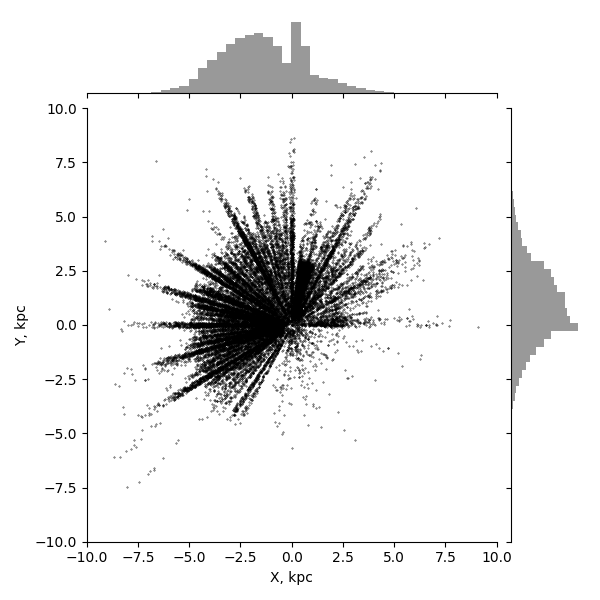
\includegraphics[width=0.95\textwidth]{../imgs/XYobj.png}
\end{minipage}
\hfill
\begin{minipage}[h]{0.49\linewidth}
        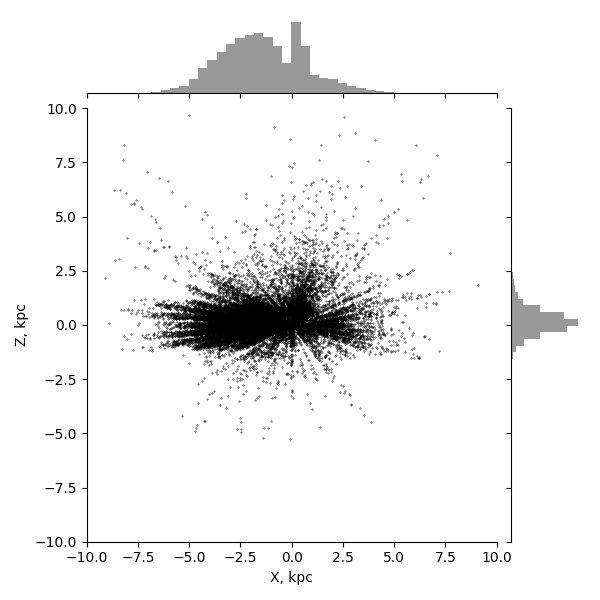
\includegraphics[width=0.95\textwidth]{../imgs/XZobj.png}
\end{minipage}
\caption{Распределение объектов APOGEE-RC в гeлиоцентрических декартовых координатах. Ось $X$ ориентирована на Центр Галактики. }
\end{figure}


\pagebreak

\begin{figure}[h!]
\begin{minipage}[h]{1.0\linewidth}
        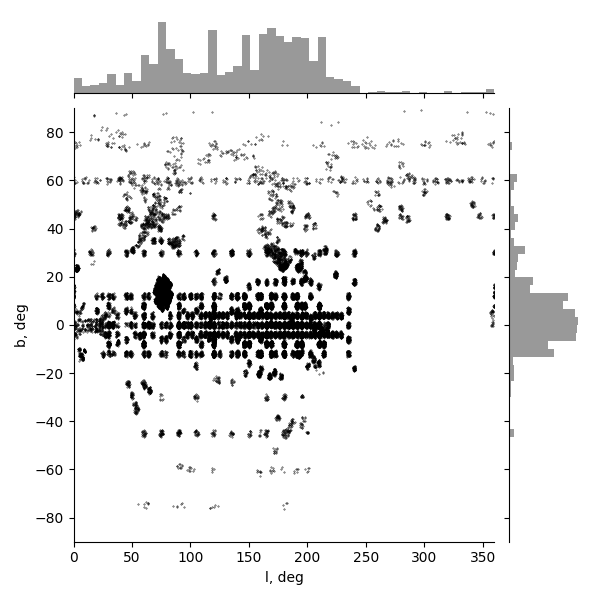
\includegraphics[width=0.95\textwidth]{../imgs/lb.png}
\end{minipage}
\caption{Распределение объектов в галактических координатах.}
\end{figure}

\pagebreak
\subsubsection*{Распределение ошибок скоростей:}
Лучевые скорости измерены с высокой точностью.

\begin{figure}[h!]
\begin{minipage}[h]{0.49\linewidth}
        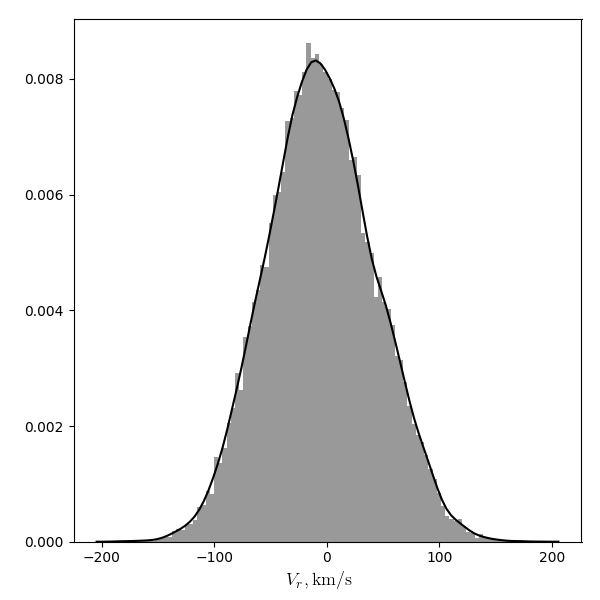
\includegraphics[width=0.95\textwidth]{../imgs/vr_distr.png}
\end{minipage}
\hfill
\begin{minipage}[h]{0.49\linewidth}
        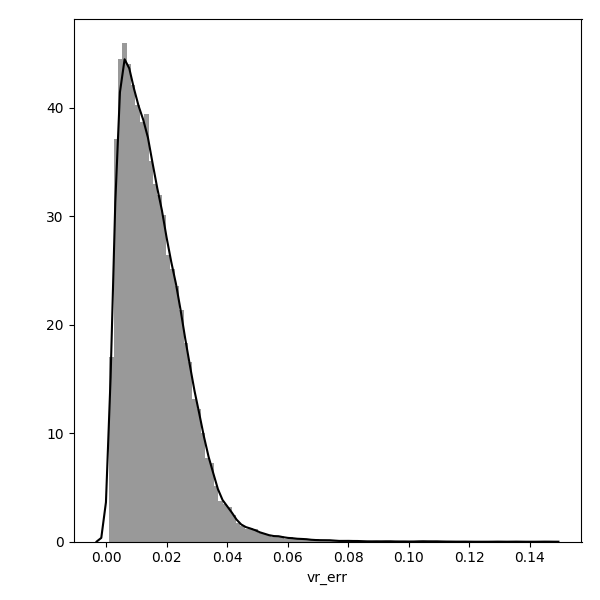
\includegraphics[width=0.95\textwidth]{../imgs/vr_err_distr.png}
\end{minipage}
\caption{Распределение лучевых скоростей и их измертельных ошибок.}
\end{figure}

\begin{figure}[h!]
\begin{minipage}[h]{0.49\linewidth}
        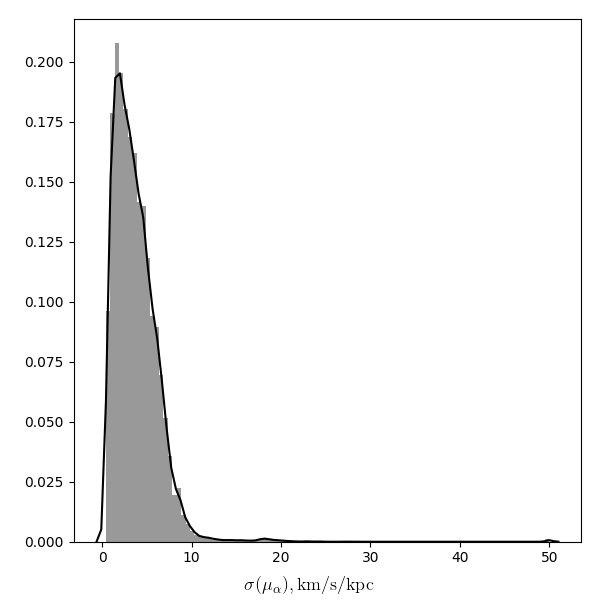
\includegraphics[width=0.95\textwidth]{../imgs/pm_ra_err_distr.png}
\end{minipage}
\hfill
\begin{minipage}[h]{0.49\linewidth}
        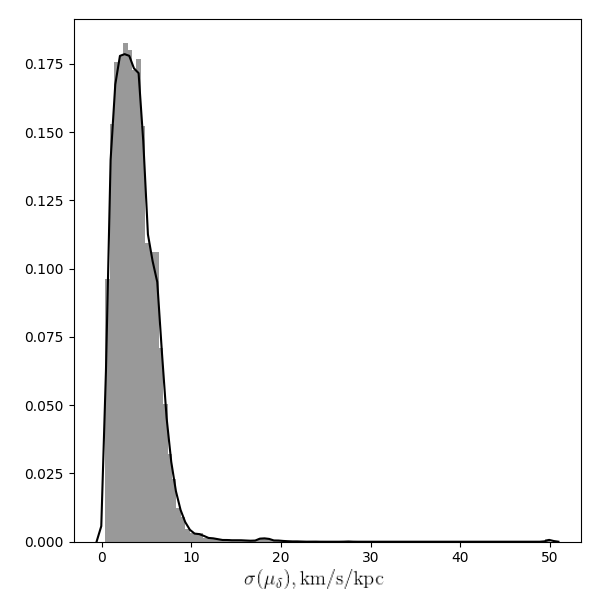
\includegraphics[width=0.95\textwidth]{../imgs/pm_dec_err_distr.png}
\end{minipage}
\caption{Распределение ошибок собственных движений в пересечении с каталогом UCAC-4.}
\end{figure}

\begin{figure}[h!]
\begin{minipage}[h]{0.49\linewidth}
        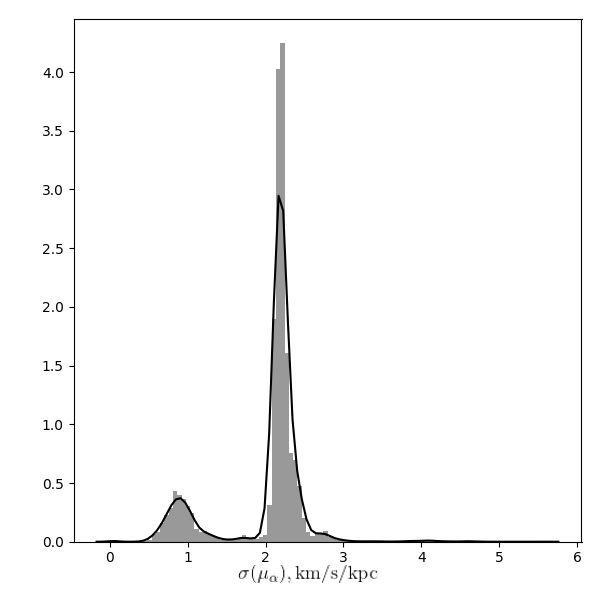
\includegraphics[width=0.95\textwidth]{../imgs/pm_ra_err_distr_hsoy.png}
\end{minipage}
\hfill
\begin{minipage}[h]{0.49\linewidth}
        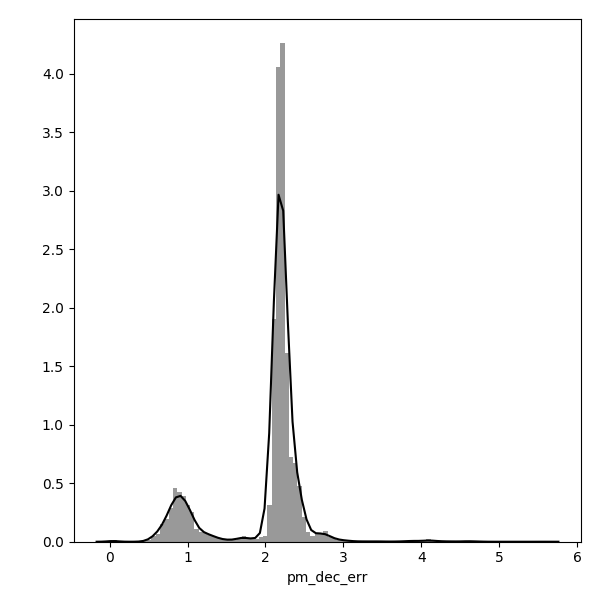
\includegraphics[width=0.95\textwidth]{../imgs/pm_dec_err_distr_hsoy.png}
\end{minipage}
\caption{Распределение ошибок собственных движений в пересечении с каталогом HSOY.}
\end{figure}

Видно, что неопределенность собственных движений объектов из каталога HSOY значительно меньше, чем для объектов из каталога UCAC-4. Наличие двух локальных максимумов распределения неопределенности сбоственных движений в пересечении с каталогом HSOY объясняется происхождением самого каталога \cite{HSOY}.
\pagebreak
\subsubsection{Переход к галактической системе координат}
\par \paragraph{Собственные движения.} 
Так как данные о собственных движениях в приводятся экваториальной СК, нужно было осуществить преобразование $(\mu_{\alpha}, \mu_{\delta}) \rightarrow (\mu_l, \mu_b)$.
\begin{equation}
        \sin{b} = \sin{\delta} \cos(90^{\circ} - \delta_p) - \cos{\delta} \sin(\alpha - \alpha_p - 90^{\circ}) \sin(90^{\circ} - \delta_p),
\end{equation}
\begin{equation}
        \sin{\varphi} = \frac{\cos{\delta} \sin(\alpha - \alpha_p - 90^{\circ}) \cos(90^{\circ} - \delta_p) + \sin{\delta} \sin(90^{\circ} - \delta_p)}{\cos{b}},
\end{equation}
\begin{equation}
        \cos{\varphi} = \frac{ \cos{\delta} \cos(\alpha - \alpha_p - 90^{\circ})}{\cos{b}},
\end{equation}
\begin{equation}
        l = \varphi + \theta_p,
\end{equation}
где $\theta_p = 32.93192^{\circ}$, $\alpha_p = 192.85948^{\circ}$, $\delta_p = 27.12825^{\circ}$ (см. \cite{ReidSolo}, appendix). Переход к собственным движениям в галактической СК:
\begin{equation}
        \mu_l = l(\alpha + \mu_{\alpha}, \delta + \mu_{\delta}) - l(\alpha, \delta),
\end{equation}
\begin{equation}
        \mu_b = b(\alpha + \mu_{\alpha}, \delta + \mu_{\delta}) - b(\alpha, \delta).
\end{equation}
Также необходимо подставлять в (\ref{l_sys}) $\mu_l^* = \mu_l \cos{b}$.

\par \paragraph{Ошибки собственных движений.} 
\par Так как в каталогах UCAC-4 и HSOY указаны ошибки собственных движений в экваториальных координатах, необходимо также привести их к галактической СК. Для этого используется формула распространения ошибок \cite{Agekyan}:
\begin{equation}
        \sigma_{\mu_{(l, b)}} = \sqrt{\left(\frac{\partial \mu_{(l, b)}}{\partial \alpha} \sigma_{\mu_{\alpha}} \right)^2 + \left(\frac{\partial \mu_{(l, b)}}{\partial\delta} \sigma_{\mu_{\delta}} \right)^2}.
\end{equation}


\begin{table}[h!]
\centering
\caption{Наблюдательные данные (приведены на эпоху \texttt{J2000})}
\begin{tabular}{|l|l|l|}
\hline
\textbf{Величина} & \textbf{Обозначение} & \textbf{Ед. изм.} \\
\hline
Прямое восхождение & $\alpha$ & deg \\
Склонение & $\delta$ & deg \\
Галактическая долгота & $l$ & deg \\
Галактическая широта & $b$ & deg \\
\hline
Гелиоцентрическая лучевая скорость & $V_{r, \mathrm{obs}}$ & km/s \\
Ошибка лучевой скорости & $\sigma_{V_{r, i}}$ & km/s \\
Гелиоцентрическое расстояние & $r$ & kpc \\
\hline
Проекция собственного движения по $\alpha$  & $\mu_{\alpha}* \cos{\delta}$ & mas/yr \\
Собственное движение по $\delta$  & $\mu_{\delta}$ & mas/yr \\
Ошибка собственного движения по $\alpha$  & $\sigma_{\mu_{\alpha}, i}$ & mas/yr \\
Ошибка собственного движения по $\delta$  & $\sigma_{\mu_{\delta}, i}$ & mas/yr \\
\hline
\end{tabular}
\end{table}


\subsubsection{Формирование выборок для оценки ошибок параметров методом \\ Монте-Карло} \label{mk}
Несмотря на то, что при частном решении используется обычный МНК, получать из матрицы ковариаций ошибки параметров некорректно, так как производится оптимизация по нелинейному параметру. Для того, чтобы исключить смещение и обеспечить состоятельность и эффектривность оценки ошибков параметров модели, используется метод Монте-Карло. Для получения ошибок параметров при решении (\ref{v_r_sys}) - (\ref{l_sys}), а также (\ref{chi_sq_func}), формируются псевдослучайные каталоги. В каждом из них такие же сведения о $l$, $b$, $r$, как в оригинальном APOGEE-RC ($\alpha$ и $\delta$ для решения систем не нужны). Лучевые скорости и собственные движения получались как
\begin{equation}
        V_{r, i}^{*} \in \mathcal{N} \left[ V_{r, \mathrm{mod}}(l_i, b_i, r_i), ~\sigma^2_{V_r} \right],
\end{equation}
\begin{equation}
        \mu_{b, i}^{*} \in \mathcal{N} \left[ \mu_{b, \mathrm{mod}}(l_i, b_i, r_i), ~\sigma^2_{\mu_b} \right],
\end{equation}
\begin{equation}
        \mu_{l, i}^{*} \in \mathcal{N} \left[ \mu_{l, \mathrm{mod}}(l_i, b_i, r_i), ~\sigma^2_{\mu_l} \right].
\end{equation}
\par После этого для каждого каталога находятся все параметры модели и строится кривая вращения. По совокупности всех найденных значений производится окончательная оценка параметров и построение доверительных областей кривой вращения.

\par В варианте с учетом природной дисперсии распределения лучевых скоростей и собственных движений приобретают вид
\begin{equation}
        V_{r, i}^{*} \in \mathcal{N} \left[ V_{r, \mathrm{mod}}(l_i, b_i, r_i),  ~\sigma^2_{V_{r, i}} + \sigma^2_0\right],
\end{equation}
\begin{equation}
        \mu_{b, i}^{*} \in \mathcal{N} \left[ \mu_{b, \mathrm{mod}}(l_i, b_i, r_i),  ~k \sigma^2_{\mu_{b, i}} + \frac{\sigma_0^2}{r^2_i} \right],
\end{equation}
\begin{equation}
        \mu_{l, i}^{*} \in \mathcal{N} \left[ \mu_{l, \mathrm{mod}}(l_i, b_i, r_i), ~k \sigma^2_{\mu_{l, i}} + \frac{\sigma_0^2}{r^2_i} \right].
\end{equation}

\subsubsection{Оценка неопределенности расстояния до центра Галактики} \label{err_r0}
Для нахождения доверительных интервалов нелинейного параметра модели $R_0$ используем следующий метод \cite{Agladze}. Для целевых функций
\begin{equation}
        S^2(R_0) = \sum_{i=1}^N \frac{\left(V_{\mathrm{mod}}(R_0) - V_{\mathrm{obs}} \right)^2_i}{\sigma_i^2}
\end{equation}
рассмотрим статистики 
\begin{equation}
        \zeta^2_0 \equiv \frac{1}{N_{\mathrm{free}}} \mathrm{min} S^2(R_0) = \frac{1}{N_{\mathrm{free}}} S^2(R_0^{\mathrm{opt}}).
\end{equation}
Границами доверительного интервала параметра $R_0$ с уровнем $s \sigma$ (мы берем стандартное значение $s = 1$) будут корни уравнения
\begin{equation} \label{dovint}
        \zeta^2_1(R_0) = \zeta_0^2 \left( 1 + \frac{s^2}{N_{\mathrm{free}}} \right).
\end{equation}
Несимметричные профили для $R_0$ приводят к тому, что оценки снизу и сверху отличаются. В результатах приводятся обе границы доверительного интервала. 


\begin{figure}[h!]
        \begin{center}
\begin{minipage}[h]{0.4\linewidth}
        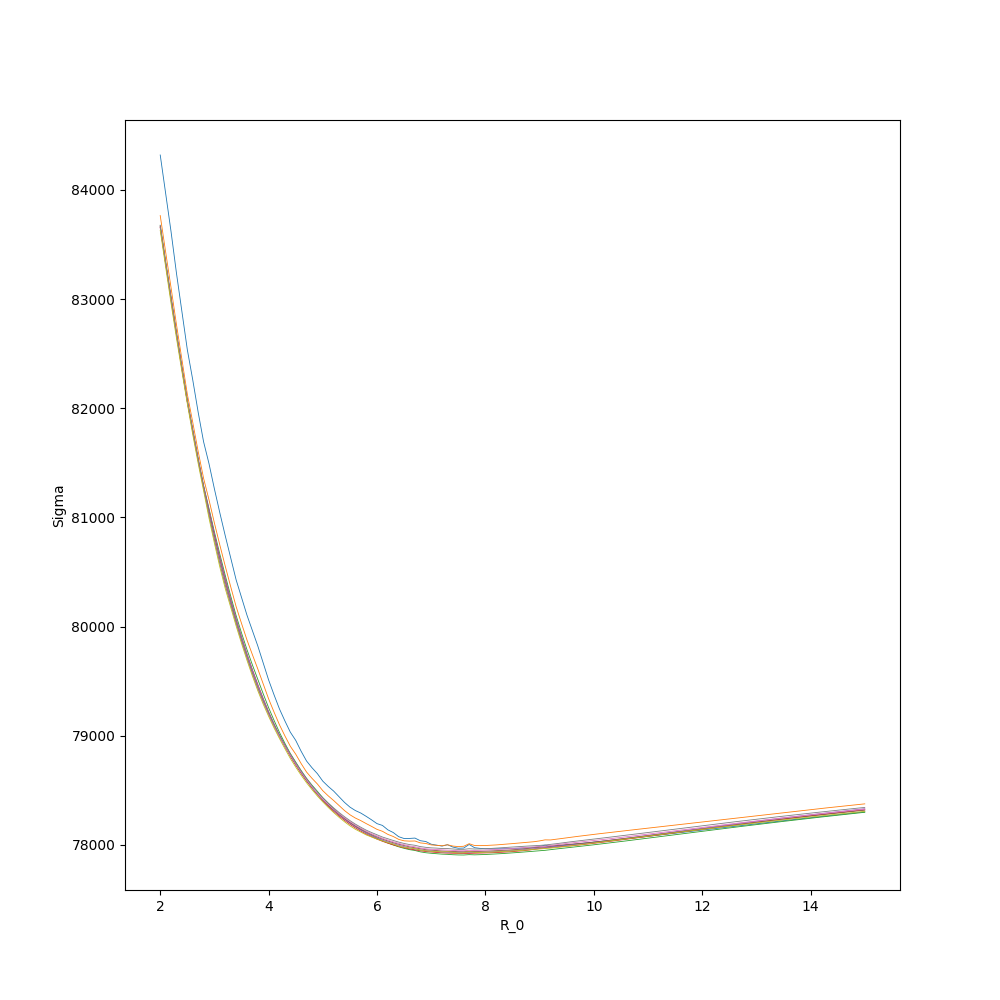
\includegraphics[width=0.95\textwidth]{../imgs/profiles.png}
\end{minipage}
        \caption{Пример профилей целефой функции для параметра $R_0$, описанной в \ref{united_mod_section}.}
        \end{center}
\end{figure}

Видно, что для некоторых (младших) порядков профили целевой функции могут быть существенно негладкими, т.е. попытка определить формальные доверительные интервалы с помощью (\ref{dovint}) приведет к тому, что уровень $\zeta_1^2(R_0)$ будет пересечен более двух раз. В таком случае более достоверными могут являться оценки неопределенности с помощью метода Монте-Карло, однако такое поведение профилей целевой функции свидетельствует в пользу того, чтобы рассмотреть более высокие порядки разложения $\Theta(R)$. 

\pagebreak
\subsection{Моделирование по лучевым скоростям} \label{vr_res}
Решается (\ref{v_r_sys}) с полным набором параметров. Порядок разложения $n < 10$. Итеративно применяется \ref{err_filter}, пока в выборке не будет объектов, попадающих под критерий (\ref{criteria}). После этого производится оценка ошибок параметров с помощью \ref{mk} по финальной выборке размера $N_{\mathrm{end}}$. Результаты приведены в таблице. 
\begin{table}[h!!]
\centering
\caption{Результаты по $V_r$.}
\begin{tabular}{r|rr|r|rrrrrr}
\hline
 $n$ & $1$ & $2$ & $3$ & $4$ & $5$&$ 6 $&$ 7 $&$ 8 $&$ 9 $\\\hline
 $N_{\mathrm{end}}$ & 29396       &   29400 &   29401 &   29401 &   29401 &   29403 &   29404 &   29404 &   29404  \\
 $R_0 $& 8.167       &   7.515 &   7.611 &   7.487 &   7.616 &   7.797 &   7.806 &   7.822 &   7.528  \\
       & $_{-0.113}^{+0.132} $ & $_{-0.052}^{+0.051}$  & $_{-0.143}^{+0.245}$   & $_{-0.075}^{+0.092}$  & $_{-0.144}^{+0.258}$  & $_{-0.064}^{+0.096}$  & $_{-0.065}^{+0.097}$  & $_{-0.070}^{+0.105}$  & $_{-0.043}^{+0.042}$  \\\hline
 $\sigma_{V_r} $& 32.189      &  32.213 &  32.117 &  32.103 &  32.096 &  32.108 &  32.117 &  32.118 &  32.112  \\
 $ u_{\odot} $& 12.412      &  12.275 &  12.688 &  12.754 &  12.785 &   12.81 &  12.807 &  12.805 &  12.814  \\
 $\sigma_{u_{\odot}} $&0.270       &   0.265 &   0.267 &   0.267 &   0.261 &   0.269 &    0.270 &   0.267 &   0.253  \\
 $v_{\odot} $& 29.601      &  28.161 &   26.98 &  27.271 &  27.098 &  27.643 &  27.769 &  27.763 &  26.871  \\
 $\sigma_{v_{\odot}}$&0.358       &   0.393 &    0.470 &   0.458 &   0.491 &   0.527 &   0.505 &   0.518 &   0.462  \\
 $w_{\odot} $&6.698       &   6.894 &    7.320 &   7.372 &   7.524 &   7.522 &   7.446 &   7.434 &   7.614  \\
 $\sigma_{w_{\odot}} $& 0.636       &   0.615 &   0.633 &   0.639 &   0.619 &    0.610 &    0.630 &   0.663 &    0.660  \\\hline
 $A $&13.013      &  12.969 &  14.491 &  15.022 &  15.279 &  15.662 &  15.612 &  15.459 &  15.345  \\
 $\sigma(A) $ & 0.128     &    0.130 &   0.174 &   0.206 &   0.209 &   0.262 &   0.262 &   0.306 &   0.318  \\
 $\theta_2$&-        &  -0.974 &  -2.038 &  -1.156 &  -1.776 &  -0.842 &  -0.549 &  -0.624 &  -2.635  \\
 $\sigma(\theta_2)$&-      &   0.169 &   0.222 &   0.279 &   0.343 &   0.423 &   0.558 &   0.536 &   0.731  \\
 $\theta_3$&-      &    - &   2.009 &   2.655 &   3.385 &   4.322 &   4.101 &   3.523 &   2.825  \\
 $\sigma(\theta_3)$&-      &    - &   0.147 &   0.192 &   0.270 &   0.403 &   0.480 &   0.814 &   0.843  \\
 $\theta_4$&-      &    - &    - &  -0.681 &  -0.184 &  -1.227 &  -1.561 &  -1.297 &   2.809  \\
 $\sigma(\theta_4)$&-      &    - &    - &   0.132 &   0.183 &   0.346 &   0.560 &   0.601 &   1.265  \\
 $\theta_5$&-      &    - &    - &    - &  -0.498 &  -0.946 &  -0.645 &   0.073 &   0.392  \\
 $\sigma(\theta_5)$&-      &    - &    - &    - &   0.132 &   0.189 &   0.423 &   0.936 &   1.017  \\
 $\theta_6$&-      &    - &    - &    - &    - &   0.521 &   0.691 &   0.224 &  -6.131  \\
 $\sigma(\theta_6)$&-    &    - &    - &    - &    - &   0.156 &   0.286 &   0.570 &   1.714  \\
 $\theta_7$&-     &    - &    - &    - &    - &    - &  -0.173 &  -0.579 &   1.354  \\
 $ \sigma(\theta_7)$&-     &    - &    - &    - &    - &    - &   0.229 &   0.539 &   0.868  \\
 $\theta_8$&-     &    - &    - &    - &    - &    - &    - &   0.340 &   5.034  \\
 $ \sigma(\theta_8)$&-     &    - &    - &    - &    - &    - &    - &   0.390 &   1.246  \\
 $\theta_9$&-     &    - &    - &    - &    - &    - &    - &    - &  -3.030  \\
 $ \sigma(\theta_9)$&-     &    - &    - &    - &    - &    - &    - &    - &   0.779  \\

\end{tabular}
\end{table}

Оценки параметров, полученные таким образом, можно сопоставлять с оценками, полученными далее по собственным движениям (в частности, будет представлять интерес поведение параметра $A$). Оптимальный порядок здесь $n = 3$, так как для более низких порядков дисперсия скоростей выше, для $n = 4$ имеем негладкие профили, для $n = 5$ имеем незначимые коэффициенты при одинаковой структуре кривой (то есть, дополнительные степени свободы уже не выявляют дополнительных деталей).
\pagebreak
\subsection{Моделирование по собственным движениям} \label{mu_res}
Решается (\ref{l_sys}) с полным набором параметров. Порядок разложения $n < 10$. Итеративно применяется \ref{err_filter}, пока в выборке не будет объектов, попадающих под критерий (\ref{criteria}). После этого производится оценка ошибок параметров с помощью \ref{mk} по финальной выборке размера $N_{\mathrm{end}}$. Результаты приведены в таблице. 
\begin{table}[h!!]
\centering
\caption{Результаты для $\mu_l$ по пересечению с каталогом UCAC-4.}
\begin{tabular}{r|rrr|rr|rrrrr}
\hline
$n$ & $1$ & $2$ & $3$ & $4$ & $5$&$ 6 $&$ 7 $&$ 8 $&$ 9 $\\\hline
 $N_{\mathrm{end}}$ & 26906       &   26906 &   26906 &   26900 &   26903 &   26904 &   26903 &   26903 &   26903 \\
 $R_0 $& 7.611       &   7.619 &   7.623 &   8.528 &   8.331 &   8.246 &   8.257 &   7.633 &   8.252 \\
       & $_{-0.328}^{+0.059} $ & $_{-0.266}^{+0.053}$ & $_{-0.213}^{+0.052}$   & $_{-0.530}^{+0.553}$  & $_{-0.450}^{+0.490}$  & $_{-0.409}^{+0.449}$  & $_{-0.476}^{+0.610}$  & $_{-0.125}^{+0.038}$  & $_{-0.435}^{+0.465}$  \\\hline
 $\sigma_{\mu_l} $& 28.038      &  28.037 &  28.038 &  27.974 &  27.998 &  28.006 &  27.995 &  27.995 &  27.995 \\
 $ u_{\odot} $& 9.679       &    9.710 &   9.697 &    9.480 &   9.507 &   9.539 &    9.490 &   9.487 &   9.438 \\
 $\sigma_{u_{\odot}} $&0.595       &   0.632 &   0.576 &   0.577 &   0.593 &   0.578 &   0.587 &    0.570 &    0.580 \\
 $v_{\odot} $& 17.940      &  17.945 &  17.709 &  17.278 &  17.657 &  17.846 &  17.985 &  18.025 &  17.831 \\
 $\sigma_{v_{\odot}}$&0.519       &   0.522 &   0.574 &   0.542 &   0.612 &   0.671 &   0.695 &   0.721 &   0.718 \\
 $\omega_0 $&24.461      &  24.417 &  24.453 &  24.446 &  24.403 &  24.387 &  24.354 &   24.37 &  24.355 \\
 $\sigma_{\omega_0} $& 0.448       &   0.477 &    0.430 &   0.447 &   0.429 &   0.449 &   0.452 &   0.457 &   0.456 \\\hline
 $A $&12.143      &  11.841 &  11.923 &  12.695 &  12.708 &  12.535 &  12.908 &  13.067 &   13.24 \\
 $\sigma(A) $ & 0.309       &   0.383 &   0.374 &   0.392 &   0.377 &   0.451 &   0.484 &   0.486 &   0.532 \\
 $\theta_2$&-        &  -0.436 &   -0.720 &  -0.389 &   0.594 &   0.741 &   1.892 &   2.783 &   2.208 \\
 $\sigma(\theta_2)$&-      &   0.279 &   0.443 &   0.412 &   0.607 &   0.632 &    0.810 &   1.157 &   1.051 \\
 $\theta_3$&-      &    - &   0.240 &   1.755 &   1.295 &   0.710 &   1.608 &   1.700 &   3.142 \\
 $\sigma(\theta_3)$&-      &    - &   0.275 &   0.352 &   0.396 &   0.769 &   0.935 &   1.199 &   1.507 \\
 $\theta_4$&-      &    - &    - &  -1.046 &  -1.560 &  -1.401 &  -3.620 &  -5.451 &  -5.339 \\
 $\sigma(\theta_4)$&-      &    - &    - &   0.202 &   0.332 &   0.351 &   0.948 &   1.502 &   1.671 \\
 $\theta_5$&-      &    - &    - &    - &  0.345 &   0.666 &   0.899 &   2.217 &  -0.558 \\
 $\sigma(\theta_5)$&-      &    - &    - &    - &   0.165 &   0.397 &   0.450 &   1.655 &   1.935 \\
 $\theta_6$&-      &    - &    - &    - &    - &   -0.160 &   1.142 &   2.101 &   4.005 \\
 $\sigma(\theta_6)$&-    &    - &    - &    - &    - &  0.172 &   0.645 &   0.802 &   2.184 \\
 $\theta_7$&-     &    - &    - &    - &    - &    - &  -0.578 &  -2.118 &  -0.459 \\
 $ \sigma(\theta_7)$&-     &    - &    - &    - &    - &    - &    0.254 &   1.345 &   1.189 \\
 $\theta_8$&-     &    - &    - &    - &    - &    - &    - &   0.525 &  -2.062 \\
 $ \sigma(\theta_8)$&-     &    - &    - &    - &    - &    - &    - &   0.525 &   1.844 \\
 $\theta_9$&-     &    - &    - &    - &    - &    - &    - &    - &  0.913 \\
 $ \sigma(\theta_9)$&-     &    - &    - &    - &    - &    - &    - &    - &   0.769 \\
\end{tabular}
\end{table}

\par Здесь оптимальный порядок $n=4$ (первые три порядка даже не дают падения дисперсии скоростей, старший коэффициент у $n=3$ незначимый, и очевидно плохой профиль целевой функции для параметра $R_0$ из-за малой формальной положительной ошибки $R_0$), и также $n =5$ может быть признан оптимальным. В таком случае, когда несколько порядков одинаково хороши, их называют как \textit{допустимые} (похожа ситуация имела место быть, например, здесь \cite{NII}).

\pagebreak
\begin{table}[h!!]
\centering
\caption{Результаты для $\mu_l$ по пересечению с каталогом HSOY}
\begin{tabular}{r|rrr|r|rrrrr}
\hline
$n$ & $1$ & $2$ & $3$ & $\textbf{4}$ & $5$&$ 6 $&$ 7 $&$ 8 $&$ 9 $\\\hline
 $N_{\mathrm{end}}$ & 28378       &   28377 &   28378 &   28378 &   28379 &   28379 &   28378 &   28378 &   28377 \\
 $R_0 $& 6.718*      &   8.185 &   8.792 &   8.694 &   8.732 &   8.726 &    8.590 &   8.744 &   8.733 \\
       & $_{-0.067}^{+0.067} $ & $_{-0.387}^{+0.462}$ & $_{-0.444}^{+0.286}$   & $_{-0.398}^{+0.337}$  & $_{-0.409}^{+0.303}$  & $_{-0.401}^{+0.312}$  & $_{-0.438}^{+0.404}$  & $_{-0.437}^{+0.307}$  & $_{-0.358}^{+0.339}$  \\\hline
 $\sigma_{\mu_l} $& 22.956      &  22.884 &  22.879 &  22.874 &  22.881 &  22.881 &  22.875 &  22.875 &  22.868  \\ 
 $ u_{\odot} $& 11.563      &  11.808 &  11.679 &  11.658 &  11.636 &   11.65 &  11.644 &  11.622 &  11.564  \\
 $\sigma_{u_{\odot}} $&0.484       &   0.492 &    0.49 &   0.493 &   0.484 &   0.487 &   0.487 &   0.497 &   0.498  \\
 $v_{\odot} $& 20.519      &  21.075 &  19.982 &  19.934 &   19.75 &  19.816 &  19.957 &   19.79 &  19.805  \\
 $\sigma_{v_{\odot}}$&0.462       &   0.429 &   0.494 &   0.498 &   0.522 &   0.576 &   0.572 &   0.601 &   0.608  \\
 $\omega_0 $&29.275      &  28.786 &  28.842 &  28.908 &  28.911 &  28.908 &  28.902 &  28.905 &  28.889  \\
 $\sigma_{\omega_0} $& 0.346       &   0.376 &   0.369 &   0.373 &   0.364 &   0.363 &   0.366 &   0.371 &   0.368  \\\hline
 $A $&15.953      &  13.636 &  13.988 &  14.447 &  14.456 &  14.395 &  14.495 &  14.604 &  14.705  \\
 $\sigma(A) $ & 0.234       &   0.295 &   0.307 &   0.333 &   0.325 &   0.364 &   0.378 &    0.420 &   0.442  \\
 $\theta_2$&-        &  -3.161 &  -4.465 &  -3.917 &  -4.185 &  -4.152 &  -3.642 &  -3.959 &  -3.627  \\
 $\sigma(\theta_2)$&-      &    0.209 &   0.321 &   0.359 &   0.463 &   0.489 &   0.685 &   0.693 &   0.748  \\
 $\theta_3$&-      &    - &   1.075 &   1.643 &   1.785 &   1.598 &   1.729 &   2.329 &   2.652  \\
 $\sigma(\theta_3)$&-      &    - &   0.203 &   0.252 &   0.298 &   0.585 &   0.668 &   0.925 &   1.117  \\
 $\theta_4$&-      &    - &    - &  -0.527 &  -0.398 &  -0.337 &  -1.051 &  -0.870 &  -1.692  \\
 $\sigma(\theta_4)$&-      &    - &    - &    0.148 &   0.235 &   0.266 &   0.743 &   0.774 &   1.196  \\
 $\theta_5$&-      &    - &    - &    - &  -0.096 &  -0.005 &   0.163 &  -0.639 &  -0.744  \\
 $\sigma(\theta_5)$&-      &    - &    - &    - &    0.126 &   0.292 &   0.337 &   0.990 &   1.157  \\
 $\theta_6$&-      &    - &    - &    - &    - &   -0.048 &   0.327 &   0.472 &   1.466  \\
 $\sigma(\theta_6)$&-    &    - &    - &    - &    - &   0.131 &   0.435 &   0.448 &   1.492  \\
 $\theta_7$&-     &    - &    - &    - &    - &    - &  -0.183 &   0.278 &   0.035  \\
 $ \sigma(\theta_7)$&-     &    - &    - &    - &    - &    - &     0.189 &   0.634 &   0.633  \\
 $\theta_8$&-     &    - &    - &    - &    - &    - &    - &   -0.225 &  -0.792  \\
 $ \sigma(\theta_8)$&-     &    - &    - &    - &    - &    - &    - &    0.286 &   1.051  \\
 $\theta_9$&-     &    - &    - &    - &    - &    - &    - &    - &  0.303  \\
 $ \sigma(\theta_9)$&-     &    - &    - &    - &    - &    - &    - &    - &   0.470  \\
\end{tabular}
\end{table}

\par Здесь также оптимален порядок с $n=4$ (для младших порядков профили существенно менее гладкие, для более старших имеем незначимость старших коэффициентов). Кажещееся улучшение ситуации со значимостью старших коэффициентов при приближении к $n=9$ обманчиво, так как в таком случае уже имеют место быть краевые эффекты. Видно, что значения $A$ по лучевым скоростям лучше согласованы с результатами по пересечению с каталогом HSOY.

Аналогичного отдельного решения для системы (\ref{b_sys}) получить не удалось, так как профиль целевой функции для параметра $R_0$ в этом случае не имеет минимума на разумных $R_0$. В целом система (\ref{b_sys}) нужна для уточнения компоненты $w_{\odot}$ остаточного движения Солнца при уже заданном $R_0$.

\pagebreak
\subsection{Трехмерное поле скоростей}
\subsubsection{Результаты при игнорировании индивидуальных ошибок \\ измерения компонент скоростей}
Вариант решения, описанного в \ref{united_mod}. Порядок разложения $n < 10$. Итеративно применяется \ref{err_filter} для всех компонент -- модельных лучевых скоростей и собственных движений. После этого производится оценка ошибок параметров с помощью \ref{mk} по финальной выборке размера $N_{\mathrm{end}}$. Результаты приведены в таблице. 
\begin{table}[h!!]
\centering
\caption{APOGEE-RC с собственными движениями из UCAC-4.}
\begin{tabular}{r|rr|rrr|rrrr}
\hline
$n$ & $1$ & $2$ & $3$ & $\textbf{4}$ & $5$&$ 6 $&$ 7 $&$ 8 $&$ 9 $\\\hline
 $N_{\mathrm{end}}$ & 26477       &    26481 &    26472 &    26473 &    26473 &    26475 &    26475 &    26475 &    26475 \\
 $R_0 $&  \textbf{8.144}       &   \textbf{ 7.514} &    \textbf{7.578} &    \textbf{7.682} &  \textbf{   7.580} &  \textbf{  7.581} &  \textbf{  7.555} &  \textbf{  7.543} &  \textbf{  7.529} \\
       & $_{-0.044}^{+0.043} $ & $_{-0.023}^{+0.023}$ & $_{-0.032}^{+0.034}$   & $_{-0.039}^{+0.047}$  & $_{-0.034}^{+0.037}$  & $_{-0.035}^{+0.039}$  & $_{-0.031}^{+0.033}$  & $_{-0.029}^{+0.031}$  & $_{-0.026}^{+0.029}$  \\\hline
 $\sigma_{V_r} $& 32.223      &  32.283 &  32.178 &  32.179 &  32.171 &  32.181 &  32.194 &  32.197 &  32.195  \\ 
 $\sigma_{\mu_l} $& 27.430      &  27.402 &  27.367 &  27.378 &  27.389 &  27.398 &  27.394 &  27.391 &  27.389  \\
 $\sigma_{\mu_b} $& 24.842      &  24.828 &  24.832 &  24.827 &  24.819 &  24.820 &  24.814 &  24.814 &  24.813  \\\hline 
 $\sigma_{\Theta} $& 71.097      &  71.274 &  71.188 &  70.901 &  70.870 &  70.887 &  70.855 &  70.864 &  70.833  \\\hline 
 $ u_{\odot} $& 12.658      &   12.542 &   12.695 &   12.715 &   12.712 &   12.721 &   12.737 &   12.737 &   12.736 \\
 $\sigma_{u_{\odot}} $&0.245       &    0.236 &    0.244 &    0.246 &    0.245 &    0.255 &    0.249 &    0.257 &    0.241 \\
 $v_{\odot} $& 25.794      &   24.875 &   23.944 &   24.122 &   23.896 &   23.899 &    24.08 &   24.198 &   24.124 \\
 $\sigma_{v_{\odot}}$&0.266       &    0.295 &    0.322 &    0.326 &    0.352 &    0.328 &    0.346 &    0.339 &    0.345 \\
 $w_{\odot} $& 6.618       &    6.618 &      6.600 &    6.615 &    6.613 &     6.610 &    6.604 &    6.605 &    6.611 \\
 $\sigma_{w_{\odot}}$&0.265       &    0.258 &    0.265 &    0.264 &    0.268 &    0.259 &    0.273 &    0.272 &    0.272 \\
 $\omega_0 $&27.510      &   27.803 &   28.142 &   28.114 &   28.194 &   28.193 &   28.205 &   28.177 &   28.162 \\
 $\sigma_{\omega_0} $& 0.247       &    0.251 &    0.249 &    0.247 &     0.260 &    0.254 &     0.260 &    0.257 &    0.246 \\\hline
 $A $&12.969      &   12.641 &   13.371 &   13.636 &   13.732 &   13.741 &   13.917 &   13.771 &   13.503 \\
 $\sigma(A) $ & 0.126       &    0.141 &    0.158 &    0.198 &      0.200 &    0.216 &     0.240 &    0.239 &    0.256 \\
 $\theta_2$&-        &  -1.144 &   -2.135 &    -1.650 &   -2.062 &    -2.090 &   -1.276 &   -0.925 &   -1.432 \\
 $\sigma(\theta_2)$&-      &    0.147 &    0.191 &    0.228 &    0.288 &    0.307 &    0.464 &    0.493 &    0.572 \\
 $\theta_3$&-      &    - &   1.213 &    1.580 &    1.867 &    1.931 &    2.167 &    1.396 &    0.176 \\
 $\sigma(\theta_3)$&-      &    - &   0.124 &    0.190 &    0.219 &    0.344 &    0.358 &    0.549 &    0.702 \\
 $\theta_4$&-      &    - &    - &  -0.372 &   -0.131 &   -0.146 &   -1.350 &   -1.660 &   -0.058 \\
 $\sigma(\theta_4)$&-      &    - &    - &    0.116 &    0.164 &    0.227 &    0.528 &    0.558 &    0.913 \\
 $\theta_5$&-      &    - &    - &    - &  -0.202 &   -0.232 &    0.027 &    1.158 &    2.614 \\
 $\sigma(\theta_5)$&-      &    - &    - &    - &    0.097 &    0.175 &    0.210 &    0.683 &    0.836 \\
 $\theta_6$&-      &    - &    - &    - &    - &   0.015 &    0.676 &    0.557 &   -2.287 \\
 $\sigma(\theta_6)$&-    &    - &    - &    - &    - &   0.099 &    0.284 &    0.295 &    1.148 \\
 $\theta_7$&-     &    - &    - &    - &    - &    - &  -0.331 &   -1.047 &   -1.254 \\
 $ \sigma(\theta_7)$&-     &    - &    - &    - &    - &    - &     0.135 &    0.444 &    0.475 \\
 $\theta_8$&-     &    - &    - &    - &    - &    - &    - &   0.336 &    2.521 \\
 $ \sigma(\theta_8)$&-     &    - &    - &    - &    - &    - &    - &    0.196 &    0.843 \\
 $\theta_9$&-     &    - &    - &    - &    - &    - &    - &    - &  -0.965  \\
 $ \sigma(\theta_9)$&-     &    - &    - &    - &    - &    - &    - &    - &   0.372  \\
\end{tabular}
\end{table}

Допустимые $n = 3 .. 5$.
\pagebreak
%\begin{figure}[h!!]
%\caption{Кривая вращения для порядка $n=4$.}
%
%
%\begin{center}
%\begin{minipage}[h!!]{0.55\linewidth}
%        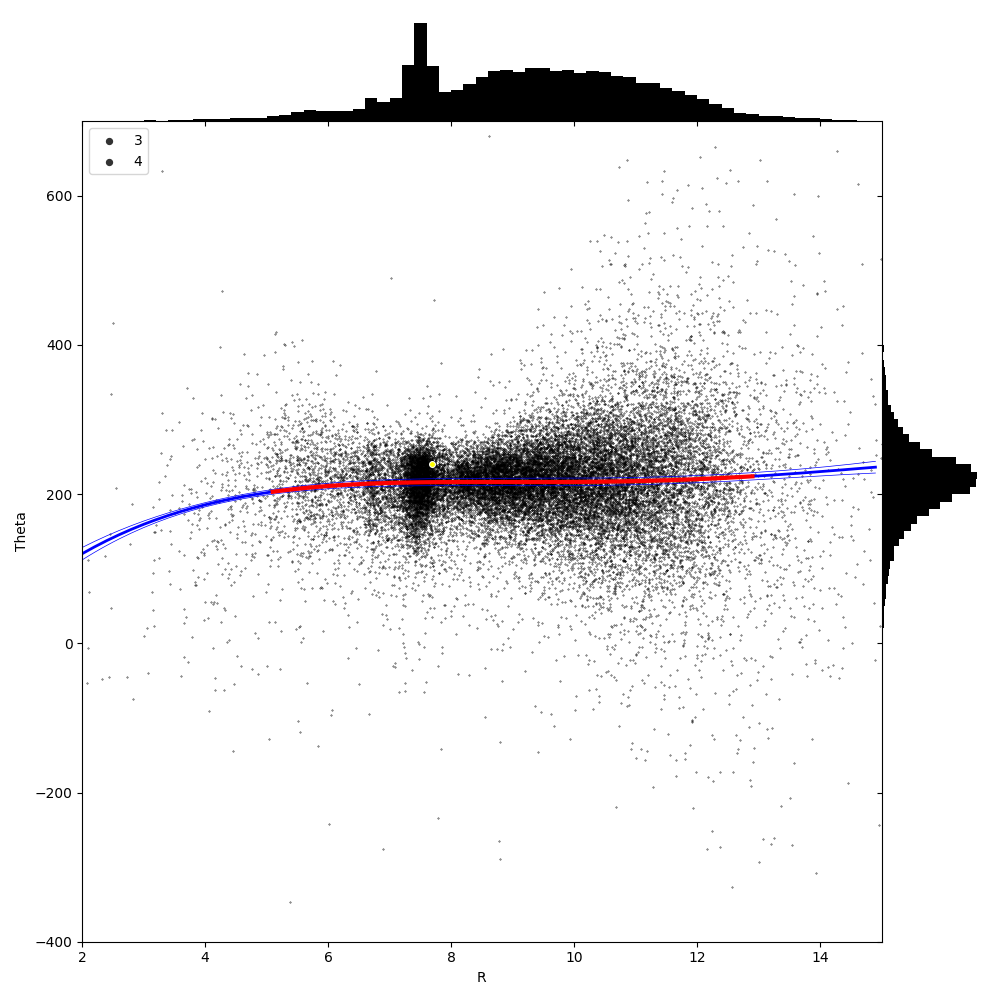
\includegraphics[width=1.0\textwidth]{../imgs/u_exc/theta_obj.png}
%\end{minipage}
%\begin{minipage}[h!!]{0.50\linewidth}
%        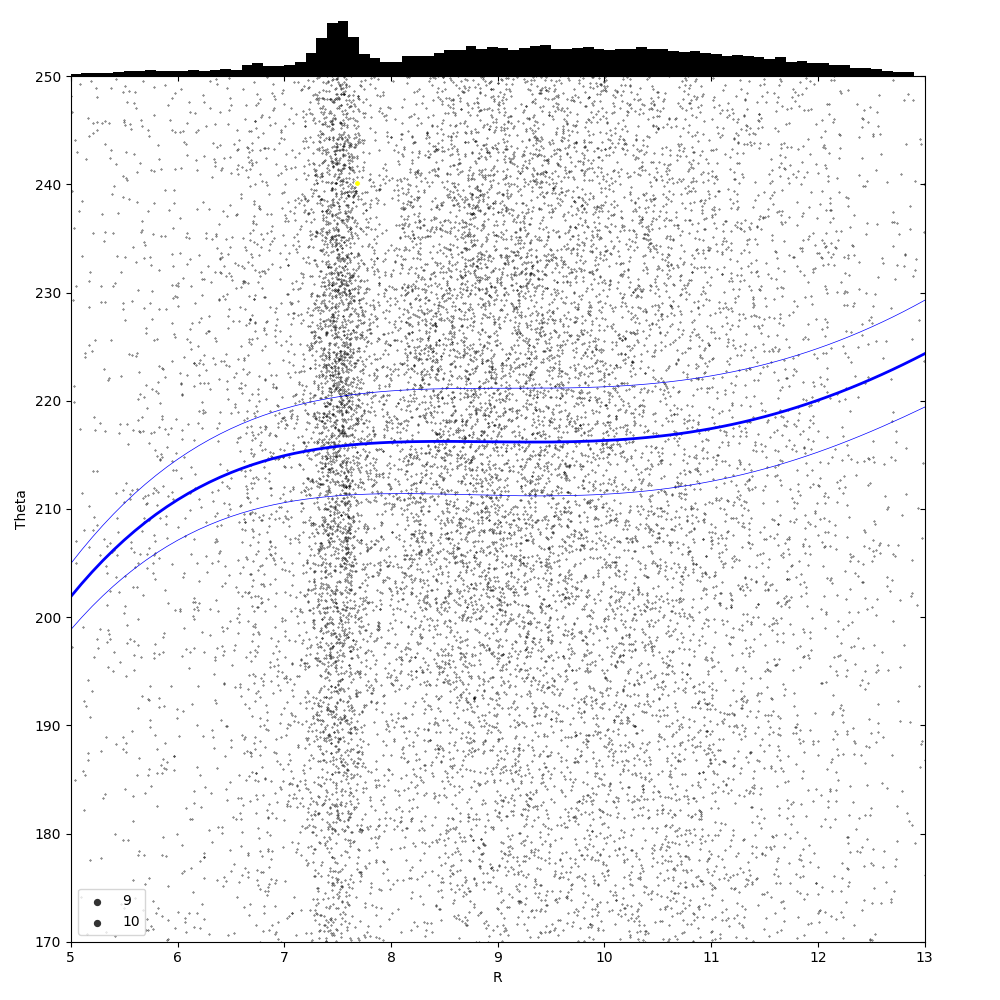
\includegraphics[width=1.0\textwidth]{../imgs/u_exc/zoomed.png}
%\end{minipage}
%\end{figure}
%\end{center}
%
%
\pagebreak

\begin{table}[h!]
\centering
\caption{APOGEE-RC с собственными движениями из HSOY.}
\begin{tabular}{r|rrrr|r|rrrr}
\hline
$n$ & $1$ & $2$ & $3$ & $\textbf{4}$ & $5$&$ 6 $&$ 7 $&$ 8 $&$ 9 $\\\hline
 $N_{\mathrm{end}}$ & 27954       &    27972 &    27968 &    27967 &   27967 &    27967 &    27968 &    27970 &    27972 \\
 $R_0 $&  \textbf{7.516}       &    \textbf{6.816} &    \textbf{6.845} &    \textbf{6.854} &   \textbf{6.849} &     \textbf{6.85} &    \textbf{6.841} &    \textbf{6.836} &    \textbf{6.828} \\
       & $_{-0.044}^{+0.043} $ & $_{-0.023}^{+0.023}$ & $_{-0.032}^{+0.034}$   & $_{-0.039}^{+0.047}$  & $_{-0.034}^{+0.037}$  & $_{-0.035}^{+0.039}$  & $_{-0.031}^{+0.033}$  & $_{-0.029}^{+0.031}$  & $_{-0.026}^{+0.029}$  \\\hline
 $\sigma_{V_r} $& 31.937      &  32.020 &  31.944 &  31.943 &  31.939 &  31.939 &  31.947 &  31.959 &  31.969  \\ 
 $\sigma_{\mu_l} $& 22.560      &  22.480 &  22.475 &  22.468 &  22.469 &  22.468 &  22.466 &  22.462 &  22.470  \\
 $\sigma_{\mu_b} $& 19.794      &  19.819 &  19.810 &  19.808 &  19.810 &  19.810 &  19.810 &  19.821 &  19.821  \\\hline 
 $\sigma_{\Theta} $& 53.454      &  52.836 &  53.124 &  52.896 &  52.743 &  52.736 &  52.772 &  52.793 &  52.773  \\\hline 
 $ u_{\odot} $& 12.373      &    12.140 &    12.320 &   12.322 &  12.324 &   12.322 &   12.332 &   12.308 &   12.309 \\
 $\sigma_{u_{\odot}} $&0.217       &    0.214 &    0.223 &    0.229 &    0.230 &    0.227 &    0.235 &    0.219 &    0.213 \\
 $v_{\odot} $& 26.731      &   25.036 &   24.163 &   24.244 &  24.082 &   24.088 &   24.313 &   24.455 &   24.454 \\
 $\sigma_{v_{\odot}}$&0.250       &    0.257 &     0.280 &    0.273 &   0.278 &    0.307 &    0.289 &    0.309 &     0.320 \\
 $w_{\odot} $& 8.371       &    8.331 &    8.323 &    8.316 &   8.319 &    8.321 &    8.315 &    8.337 &    8.345 \\
 $\sigma_{w_{\odot}}$&0.219       &     0.220 &     0.210 &    0.222 &   0.215 &    0.217 &    0.218 &    0.215 &    0.213 \\
 $\omega_0 $&27.767      &   28.344 &   28.685 &   28.689 &  28.729 &    28.72 &   28.714 &   28.683 &   28.656 \\
 $\sigma_{\omega_0} $& 0.201       &    0.205 &    0.193 &    0.212 &   0.215 &     0.210 &    0.207 &    0.204 &    0.209 \\\hline
 $A $&13.741      &   12.998 &   13.676 &    13.87 &  13.923 &   13.869 &   14.096 &   13.977 &   13.555 \\
 $\sigma(A) $ & 0.114       &     0.12 &    0.137 &    0.172 &    0.170 &    0.191 &    0.186 &    0.215 &    0.243 \\
 $\theta_2$&-        &  -2.31 &   -3.196 &    -2.890 &  -3.168 &     -3.200 &   -2.262 &   -1.819 &   -2.148 \\
 $\sigma(\theta_2)$&-      &    0.127 &    0.154 &    0.194 &   0.253 &    0.275 &    0.382 &    0.462 &    0.498 \\
 $\theta_3$&-      &    - &   1.055 &    1.318 &   1.506 &    1.384 &    1.749 &    1.062 &   -1.099 \\
 $\sigma(\theta_3)$&-      &    - &   0.115 &    0.161 &   0.194 &    0.298 &    0.317 &    0.523 &    0.700 \\
 $\theta_4$&-      &    - &    - &  -0.258 &  -0.090 &   -0.028 &   -1.434 &   -1.937 &   -0.207 \\
 $\sigma(\theta_4)$&-      &    - &    - &     0.104 &   0.158 &    0.194 &    0.446 &    0.556 &    0.773 \\
 $\theta_5$&-      &    - &    - &    - &   -0.138 &   -0.070 &    0.140 &    1.296 &    4.468 \\
 $\sigma(\theta_5)$&-      &    - &    - &    - &    0.092 &    0.168 &    0.184 &    0.707 &    0.937 \\
 $\theta_6$&-      &    - &    - &    - &    - &    -0.045 &    0.793 &    0.814 &   -3.372 \\
 $\sigma(\theta_6)$&-    &    - &    - &    - &    - &    0.089 &    0.266 &    0.279 &    1.090 \\
 $\theta_7$&-     &    - &    - &    - &    - &    - &  -0.397 &   -1.222 &   -2.415 \\
 $ \sigma(\theta_7)$&-     &    - &    - &    - &    - &    - &      0.121 &    0.504 &    0.557 \\
 $\theta_8$&-     &    - &    - &    - &    - &    - &    - &   0.361 &    4.226 \\
 $ \sigma(\theta_8)$&-     &    - &    - &    - &    - &    - &    - &    0.215 &    0.949 \\
 $\theta_9$&-     &    - &    - &    - &    - &    - &    - &    - &  -1.571  \\
 $ \sigma(\theta_9)$&-     &    - &    - &    - &    - &    - &    - &    - &   0.390  \\
\end{tabular}
\end{table}

Здесь оптимален $n = 5$ (младше -- плохие профили и большая дисперсия, выше -- краевые эффекты и утрата значимости коэффициентов).
%\pagebreak
%        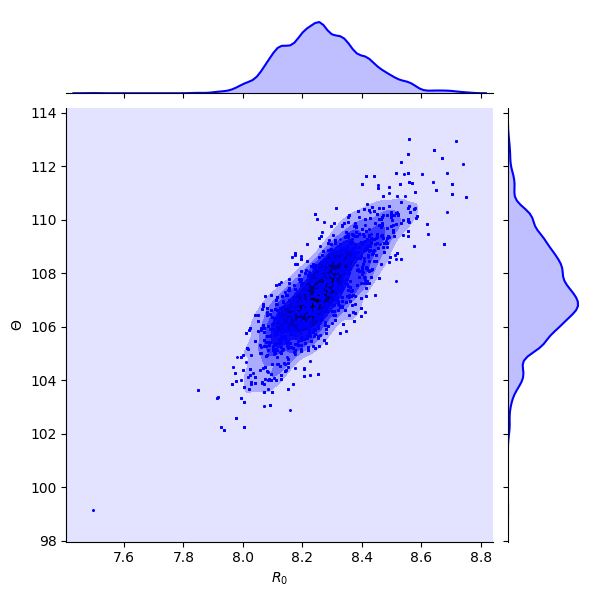
\includegraphics[width=0.9\textwidth]{../../sources/scripts/out.png}
%\pagebreak

\pagebreak

\subsubsection{Результаты с учетом природной дисперсии} \label{sigma_0_mode_section}
Вариант решения, описанного в \ref{sigma_0_mode}. Порядок разложения $n < 10$. Итеративно применяется \ref{err_filter} для всех компонент -- модельных лучевых скоростей и собственных движений. После этого производится оценка ошибок параметров с помощью \ref{mk} по финальной выборке размера $N_{\mathrm{end}}$. Результаты приведены в таблице. 
\begin{table}[h!!]
\centering
\caption{APOGEE-RC с собственными движениями UCAC-4.}
\begin{tabular}{r|rrr|rrr|rrr}
\hline
$n$ & $1$ & $2$ & $3$ & $\textbf{4}$ & $5$&$ 6 $&$ 7 $&$ 8 $&$ 9 $\\\hline
 $N_{\mathrm{end}}$ & 26504       &   26507 &   26502 &   26504 &   26504 &   26506 &   26506 &   26505 &   26507 \\
 $R_0 $& \textbf{8.689}       &   \textbf{8.048} &   \textbf{7.907} &   \textbf{8.342} &   \textbf{7.879} &   \textbf{7.886} &   \textbf{7.897} &   \textbf{7.853} &   \textbf{8.008} \\
       & $_{-0.314}^{+0.191} $ & $_{-0.079}^{+0.091}$ & $_{-0.110}^{+0.156}$   & $_{-0.114}^{+0.112}$  & $_{-0.087}^{+0.119}$  & $_{-0.079}^{+0.100}$  & $_{-0.082}^{+0.102}$  & $_{-0.074}^{+0.095}$  & $_{-0.119}^{+0.144}$  \\\hline
 $\chi^2 $& 79506   &   79514 &   79498 &   79503 &   79502 &   79507 &   79506 &   79502 &   79507 \\
 $N_{\mathrm{free}} $& 79506      &  79514 &   79498 &   79503 &   79502 &   79507 &   79506 &   79502 &   79507 \\
 $\sigma_0 $& 21.335      &  21.355 &  21.313 &  21.312 &  21.301 &  21.306 &  21.304 &  21.297 &  21.308  \\ 
 $\sigma_{\Theta} $& 71.134      &  71.403 &  71.603 &  71.223 &  71.327 &  71.342 &  71.343 &  71.301 &  71.313  \\\hline 
 $ u_{\odot} $& 12.376      &  12.272 &  12.542 &  12.593 &  12.629 &  12.651 &  12.652 &  12.657 &  12.636 \\
 $\sigma_{u_{\odot}} $&0.188       &   0.182 &   0.183 &    0.180 &   0.181 &   0.184 &   0.187 &   0.192 &   0.186 \\
 $v_{\odot} $& 30.404      &  29.438 &  28.207 &  28.956 &  27.982 &  28.107 &  28.187 &  28.055 &  28.014 \\
 $\sigma_{v_{\odot}}$&0.251       &   0.274 &   0.304 &   0.309 &   0.319 &   0.317 &   0.375 &   0.318 &    0.350 \\
 $w_{\odot} $& 5.650       &   5.752 &   6.053 &   6.064 &   6.268 &   6.267 &   6.254 &   6.328 &   6.316 \\
 $\sigma_{w_{\odot}}$&0.365       &   0.348 &   0.356 &   0.358 &   0.356 &   0.349 &   0.356 &   0.367 &   0.386 \\
 $\omega_0 $&26.690      &  27.184 &  27.396 &  27.007 &  27.335 &  27.305 &  27.293 &  27.333 &  27.227 \\
 $\sigma_{\omega_0} $& 0.284       &   0.291 &   0.294 &   0.306 &    0.310 &   0.297 &   0.311 &   0.306 &   0.289 \\\hline
 $A $&12.490      &  12.382 &  13.477 &  13.896 &  14.206 &  14.493 &    14.500 &  14.726 &  14.372 \\
 $\sigma(A) $ & 0.100       &   0.098 &   0.121 &   0.143 &   0.147 &   0.166 &   0.158 &   0.188 &   0.198 \\
 $\theta_2$&-        &  -0.749 &  -1.851 &  -0.893 &  -2.079 &  -1.724 &  -1.524 &  -1.763 &  -2.574 \\
 $\sigma(\theta_2)$&-      &    0.120 &   0.147 &   0.198 &   0.237 &   0.231 &   0.361 &   0.368 &   0.447 \\
 $\theta_3$&-      &    - &   1.541 &   2.212 &   2.931 &   3.554 &   3.540 &   4.420 &   3.320 \\
 $\sigma(\theta_3)$&-      &    - &   0.097 &   0.133 &   0.166 &   0.237 &   0.258 &   0.456 &   0.465 \\
 $\theta_4$&-      &    - &    - &  -0.622 &   0.012 &  -0.468 &  -0.726 &  -0.636 &   1.391 \\
 $\sigma(\theta_4)$&-      &    - &    - &     0.083 &   0.113 &   0.165 &   0.342 &   0.363 &   0.681 \\
 $\theta_5$&-      &    - &    - &    - &  -0.503 &  -0.800 &  -0.705 &  -1.796 &  -0.759 \\
 $\sigma(\theta_5)$&-      &    - &    - &    - &     0.075 &   0.112 &   0.163 &   0.515 &   0.453 \\
 $\theta_6$&-      &    - &    - &    - &    - &   0.255 &   0.387 &   0.644 &  -2.336 \\
 $\sigma(\theta_6)$&-    &    - &    - &    - &    - &   0.076 &   0.169 &   0.207 &   0.796 \\
 $\theta_7$&-     &    - &    - &    - &    - &    - &  -0.078 &   0.529 &   0.710 \\
 $ \sigma(\theta_7)$&-     &    - &    - &    - &    - &    - &      0.088 &   0.292 &   0.254 \\
 $\theta_8$&-     &    - &    - &    - &    - &    - &    - &   -0.313 &   1.682 \\
 $ \sigma(\theta_8)$&-     &    - &    - &    - &    - &    - &    - &     0.143 &   0.510 \\
 $\theta_9$&-     &    - &    - &    - &    - &    - &    - &    - &  -0.942  \\
 $ \sigma(\theta_9)$&-     &    - &    - &    - &    - &    - &    - &    - &   0.243  \\
\end{tabular}
\end{table}
Допустимые порядки $n=4..6$. Снизу ограничены дефектами профилей и повышенной дисперсией, сверху -- значимостью старших коэффициентов.

\pagebreak
\begin{table}[h!!] \label{table_hsoy_sigma0}
\centering
\caption{APOGEE-RC с собственными движениями HSOY.}
\begin{tabular}{r|rr|r|r|r|rrrrr}
\hline
$n$ & $1$ & $2$ & $3$ & $\textbf{4}$ & $5$&$ 6 $&$ 7 $&$ 8 $&$ 9 $\\\hline
 $N_{\mathrm{end}}$ & 27995       &    28007 &   28007 &   28006 &   28004 &   28004 &    28004 &   28005 &   28007 \\
 $R_0 $& \textbf{8.509}       &     \textbf{7.520} &   \textbf{7.548} &   \textbf{7.458} &   \textbf{7.483} &   \textbf{7.539} &     \textbf{7.540} &   \textbf{7.529} &   \textbf{7.831} \\
       & $_{-0.155}^{+0.194} $ & $_{-0.040}^{+0.038}$ & $_{-0.089}^{+0.066}$   & $_{-0.050}^{+0.055}$  & $_{-0.092}^{+0.113}$  & $_{-0.117}^{+0.082}$  & $_{-0.067}^{+0.053}$  & $_{-0.029}^{+0.031} *$  & $_{-0.026}^{+0.029} *$  \\\hline
 $\chi^2 $& 83979   &  84014 &   84013 &   84009 &   84002 &   84001 &  84000 &   84002 &   84007 \\
 $N_{\mathrm{free}} $& 83979   &  84014 &   84013 &   84009 &   84002 &   84001 &  84000 &   84002 &   84007 \\
 $\sigma_0 $& 20.984      &  21.013 &  20.983 &  20.963 &  20.959 &  20.961 &  20.955 &  20.959 &  20.972  \\ 
 $\sigma_{\Theta} $& 53.154      &  53.268 &  53.873 &  53.350 &  53.323 &  53.377 &  53.281 &  53.283 &  53.345  \\\hline 
 $ u_{\odot} $& 12.410      &   12.227 &  12.473 &  12.565 &  12.575 &  12.583 &   12.604 &  12.607 &  12.594 \\
 $\sigma_{u_{\odot}} $&0.181       &     0.180 &   0.181 &   0.174 &   0.177 &   0.181 &    0.181 &   0.175 &    0.170 \\
 $v_{\odot} $& 30.372      &   28.257 &  27.145 &  27.452 &  27.204 &  27.257 &   27.641 &  27.545 &    27.800 \\
 $\sigma_{v_{\odot}}$&0.232       &    0.256 &   0.297 &   0.283 &   0.306 &   0.305 &    0.295 &   0.315 &   0.308 \\
 $w_{\odot} $& 7.148       &    7.391 &   7.659 &   7.709 &   7.774 &   7.816 &    7.768 &   7.818 &   7.768 \\
 $\sigma_{w_{\odot}}$&0.346       &    0.339 &   0.338 &   0.354 &   0.345 &   0.331 &    0.367 &   0.349 &   0.351 \\
 $\omega_0 $&25.838      &   27.008 &  26.929 &  26.847 &  26.839 &   26.790 &   26.774 &  26.798 &  26.562 \\
 $\sigma_{\omega_0} $& 0.226       &     0.230 &   0.249 &   0.231 &   0.251 &   0.244 &    0.241 &   0.235 &   0.233 \\\hline
 $A $&12.825      &   12.646 &   13.630 &  14.328 &  14.419 &  14.652 &    14.82 &  14.995 &  14.504 \\
 $\sigma(A) $ & 0.087       &    0.087 &    0.110 &   0.129 &   0.132 &   0.152 &    0.156 &   0.179 &     0.200 \\
 $\theta_2$&-        &  -1.489 &  -2.419 &  -1.474 &  -1.975 &  -1.894 &   -0.806 &  -1.117 &  -1.568 \\
 $\sigma(\theta_2)$&-      &     0.102 &    0.130 &   0.158 &   0.198 &   0.219 &     0.310 &   0.347 &    0.410 \\
 $\theta_3$&-      &    - &   1.319 &   2.163 &   2.478 &   3.086 &    3.187 &   3.943 &   2.312 \\
 $\sigma(\theta_3)$&-      &    - &   0.081 &   0.124 &   0.144 &   0.225 &    0.235 &   0.390 &   0.455 \\
 $\theta_4$&-      &    - &    - &  -0.740 &  -0.413 &  -0.634 &   -1.899 &  -1.654 &   0.162 \\
 $\sigma(\theta_4)$&-      &    - &    - &     0.072 &   0.104 &   0.133 &    0.313 &   0.347 &   0.600 \\
 $\theta_5$&-      &    - &    - &    - &  -0.240 &  -0.578 &   -0.287 &  -1.288 &   0.460 \\
 $\sigma(\theta_5)$&-      &    - &    - &    - &     0.057 &   0.113 &    0.128 &   0.452 &   0.467 \\
 $\theta_6$&-      &    - &    - &    - &    - &   0.190 &    0.862 &   0.976 &  -2.131 \\
 $\sigma(\theta_6)$&-    &    - &    - &    - &    - &   0.058 &    0.167 &   0.172 &   0.691 \\
 $\theta_7$&-     &    - &    - &    - &    - &    - &  -0.330 &   0.277 &   0.089 \\
 $ \sigma(\theta_7)$&-     &    - &    - &    - &    - &    - &      0.074 &   0.282 &   0.264 \\
 $\theta_8$&-     &    - &    - &    - &    - &    - &    - &   -0.282 &   1.902 \\
 $ \sigma(\theta_8)$&-     &    - &    - &    - &    - &    - &    - &     0.123 &   0.440 \\
 $\theta_9$&-     &    - &    - &    - &    - &    - &    - &    - &  -0.947  \\
 $ \sigma(\theta_9)$&-     &    - &    - &    - &    - &    - &    - &    - &   0.206  \\
\end{tabular}
\end{table}
Руководствуясь теми же критериям, что и в предыдущих случаях, здесь получается, что оптимальные порядки $n=3$ и $5$. Решения с $n=4, 6, 7$ имеют нарушения связности линий равной плотности маргинальных распределений. Ещё более старшие порядки имеют краевые эффекты. 
\pagebreak

\subsection{Итоговые оценки и их обсуждение.}
Исходя из результатов \ref{mu_res} относительно \ref{vr_res}, можно сделать вывод о заниженной шкале расстояний каталога APOGEE-RC. Это проявляется в явном смещении оценок $A$ из собственных долготных движений относительно оценок $A$, полученных по лучевым скоростям. При этом результаты по пересечению с каталогом HSOY лучше соотносятся с результатами, полученными по лучевым скоростям. Поэтому первый вывод -- \textit{результаты, полученные с использованием собственных движений из каталога HSOY, следует считать более релевантными действительности.} Кроме того, как можно видеть из вариантов решения в трехмерном поле скоростей, этот каталог даёт существенно меньшую дисперсию по всем компонентам и как следствие меньшую $\sigma_{\Theta}$. Вообще, это ожидаемый результат, с учетом происхождения каталога HSOY. В дальнейшем будут обсуждаться и приводиться как окончательные оценки, полученные с использованием каталога HSOY. Отношение $K_A = \frac{A_{V_r}}{A_{\mu_l}}$ даёт нам калибровочный коэффициент для расстояний. 
\par В данной работе, из-за того что есть также и оценки $R_0$, полученные как с помощью собственных долготных движений (и гелиоцентрических расстояний), так и с помощью традиционного использования лучевых скоростей, есть возможность ввести и поправочный коэффициент $K_{R_0} = \frac{R_{0, V_r}}{R_{0, \mu_l}}$. 

\par Для подобных задач моделирования кинематики подсистем ранее использовались сравнительно небольшие выборки объектов. Оценки, полученные на основе этого каталога, имеют высокую статистическую надежность. Примененный алгоритм исключения позволяет ещё больше снизить статистические ошибки, при этом не позволяя удалить из выборки необоснованно много объектов.  Однако недостатком применённых методов решения является то, что не учитывалось изменение размера и формы эллипсоида остаточных скоростей с галактоцентрическим расстоянием. Вместе с тем, в работе \cite{Rastorguev} наилучшее описание поля наблюдаемых пространственных скоростей обеспечила модель с постоянными значениями дисперсии скоростей. В этом заключается потенциал дальнейших исследований.
\begin{table}[h!!] 
\centering
\caption{$K_A$ для допустимых порядков.}
\begin{tabular}{r|rrr|r}
        $ n$ & 3 & 4 & 5 & W. mean\\
\hline
\hline
$A_{V_r} $& $14.491     $&  $  15.022$ & $ 15.279 $ & -\\
$\sigma_{A_{V_r}}$& $0.174 $    &  $0.206 $& $  0.209  $& -\\
$A_{\mu_l} $& $13.988 $    & $ 14.447$ & $14.456 $ & -\\
$\sigma_{A_{\mu_l}}$& $0.307 $    & $0.333 $& $0.325 $ & -\\
\hline
$K_A$& $1.036 $    &   $1.040 $& $ 1.057 $ & \textbf{1.044}\\
$ \sigma_{K_A}$& $0.035 $    & $0.035 $&  $0.038 $ & \textbf{0.036}
\end{tabular}
\end{table}

\par Что касается оптимальных порядков, то, несмотря на кажущееся улучшение значимости старших коэффициентов в совместных решениях (напр., в \ref{table_hsoy_sigma0}), вид кривой вращения показывает, что имеют место краевые эффекты, обусловленные излишними степенями свободы полинома.  Поэтому оптимальный порядок не может превосходить представленные в таблицах (\ref{table_hsoy_sigma0}). 
\par Ограничение снизу на оптимальный порядок проиходит из характера \textit{профилей} решения. При малых $n$ профили являются существенно менее гладкими, тогда как с ростом $n$ профили для всех вариантов решения сглаживаются. Из-за негладкости профилей теряется возможность получать из них адекватные оценки для $R_0$, и приходится прибегать к методу Монте-Карло для получения этих оценок. Вместе с тем, наименьший порядок, при котором оценки по Монте-Карло и по профилям получаются равными, служит нижним ограничением на возможный оптимальный $n$.
\par Наилучшим вариантом решения из представленных является \ref{sigma_0_mode_section}, т.к. такой подход к решению позволяет взвесить объекты выборки обратно пропорционально квадратам их ошибок измерений, что позволяет увеличить эффективность оценок регрессии \cite{Valeev}. Проблема того, что оптимальный порядок не определяется однозначно даже с учетом множества критериев, решается следующим образом. Используя взвешенное среднее (как, например, в \cite{Camarillo}):
\begin{equation}
        M = \frac{\sum_i^N \frac{M_i}{\sigma_i^2}}{\sum_i^N \frac{1}{\sigma_i^2}}, ~\sigma^2_{\mathrm{mean}} = \frac{\sum_i \frac{N_{\mathrm{free}, i}}{2 \sigma_i^2}}{\sum_i \frac{N_{\mathrm{free}, i}}{2\sigma_i^4}}, 
\end{equation}
где $M$ -- итоговая точечная оценка параметра по $N$ наблюдениям и соответствующими стандартами $\sigma_i$, можем получить по оптимальным порядками, если их несколько, окончательные параметры модели.
\par Попытка учесть систематическую погрешность шкалы расстояний -- скорректировать гелиоцентрические расстояния каталога на полученную величину $K_A$. После этого были пересчитаны результаты в варианте \ref{sigma_0_mode}, и соответствующие результаты для сравнения приведены в колонке \textrm{Corr.} (оптимальный порядок в таком случае оказался $n=3$). Для оценки систематической неопределенности оценок $R_0$ используем упомянутые смещения калибровки каталога относительно \cite{Groenewegen}. 

\begin{table}[h!!] 
\centering
\caption{Итоговые характеристики кинематической модели (\ref{table_hsoy_sigma0}, HSOY).}
\begin{tabular}{r||r|r||r|r}
        $ n$ & 3 & 5 & W. mean & \textrm{Corr.}\\
\hline
\hline
$A $& $13.630  \pm 0.174 $ &   $ 14.419 \pm 0.206 $& $ 13.959 \pm 0.185 $& $13.086 \pm 0.106$ \\ % 13.086 \pm 0.106\\
$u_{\odot} $& $12.473 \pm 0.181  $  & $ 12.575 \pm 0.177 $& $12.525 \pm 0.179  $& $ 12.452 \pm 0.169$\\
$v_{\odot} $& $27.145 \pm 0.297  $  & $ 27.204 \pm 0.306$& $27.174  \pm 0.301 $& $27.099 \pm 0.286$\\
$w_{\odot} $& $7.659  \pm 0.338 $  &  $7.774 \pm 0.345$ & $7.715 \pm 0.341$ & $7.779 \pm 0.341$\\
\hline
$R_0 $& \textbf{7.548} $^{+0.066}_{-0.089} $   &  \textbf{7.483} $^{+0.113}_{-0.092} $  & \textbf{7.516} $^{+0.072}_{-0.090} $   & \textbf{7.838} $^{0.101}_{0.088}$ \\
$\omega_0 $& $26.929  \pm 0.249 $   &  $26.839 \pm 0.251$ & $26.884 \pm 0.250 $ & $26.076 \pm 0.236$\\
$\theta_0 $& $203.260  \pm 4.065    $&  $200.836 \pm 4.619 $& $202.202 \pm 4.281 $ & $ 204.384 \pm 4.314$ \\
\hline
$\omega_{\odot} $& $30.525  \pm 0.325  $  &  $30.474 \pm 0.342 $& $30.501 \pm 0.333 $ & $29.533 \pm 0.314$ \\
\end{tabular}
\end{table}
Совокупность работ, посвященных оцениванию <<наилучшего>> значения $R_0$, а также других галактических характеристик, на основе отдельных исследований (как например, \cite{NIId,Malkin,Camarillo}), а также самые последние \cite{Gravity} открытия позволяют сравнить полученные результаты с уже имеющимися аналогичными. 
\par Из обзоров следует, что наиболее вероятное значение $R_0$ лежит около $8$ кпк, с возможной ошибкой в сотню пк, а с учетом результатов \cite{Gravity} неопределенность во второй значащей цифре пропадает (статистическая ошибка определения $R_0$ в работе \cite{Gravity} составляет 13 пк, систематическая 22 пк). Результаты, представленные в настоящей работе, как и в \cite{Gravity}, показывают, что для таких больших выборок систематические ошибки результатов превосходят статистические. Так, систематическая неопределенность $R_0$ в данной работе составляет от $247$ до $283$ кпк. 
\par Что касается кинематических параметров, то \cite{CamarilloVEL} приводит на данный момент значения $\Theta_0 = 220 \pm 10$ км/с, $\omega_0 = 27.6 \pm 1.1$ км/с/кпк. Компонента остаточной скорости Солнца $w_{\odot}$ хорошо согласуется с другими работами (напр. \cite{Baikbob, Rastorguev}), при этом оценки для этой компоненты получаются более точными, чем перечисленых работах. Также стоит подчеркнуть, что данная компонента, обычно хорошо определяемая по системам уравнений для собственных широтных движений (\ref{b_sys}), получается с хорошей точностью уже только по системе уравнений для лучевых скоростей (\ref{v_r_sys}). 
\par Ещё лучше согласуется с другими результатами полученная величина $\omega_{\odot}$ (см. \cite{Rastorguev, Baikbob}), которая представляет природный инвариант относительно опорных объектов.

\begin{figure}[h!!]

\begin{center}
\begin{minipage}[p]{0.95\linewidth}
        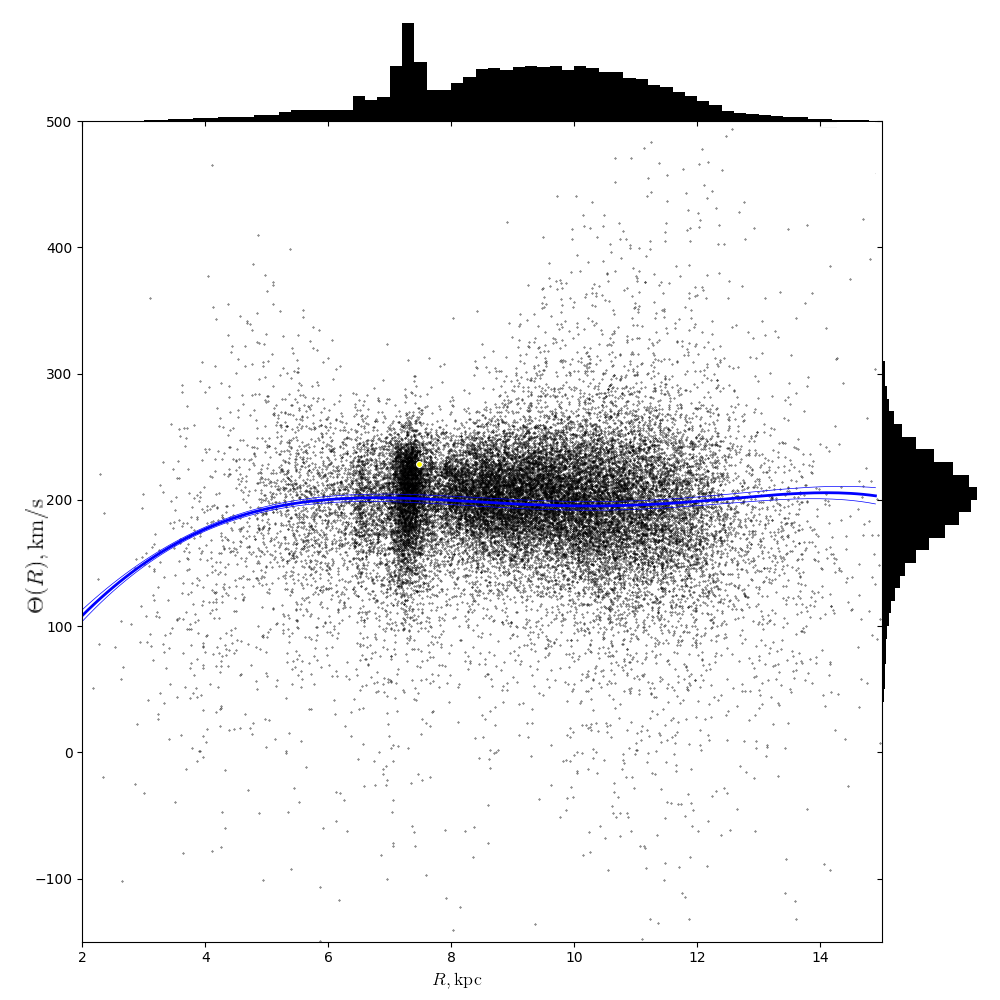
\includegraphics[width=1.0\textwidth]{../imgs/theta_obj.png}
\end{minipage}
\end{center}
\caption{Кривая вращения для порядка $n=5$. Желтый кружок -- Солнце, доверительная область для средней кривой вращения приведена для уровня $1 \sigma$, её характерная ширина на приведенном отрезке по $R \in [2, 15] ~\mathrm{кпк}$ составляет $6.5 ~\textrm{км/с}$.}
\end{figure}


\par Кривая вращения не обнаруживает мелкой структуры и плоская на всей области основного присутствия выборки. Несмотря на возможность разложения при таком объеме выборки на более высокие, чем обычно, порядки, кривая вращения не меняет принципиально своей формы при увеличении числа степеней свободы.
%\paragraph{Проверка остатков модели на нормальность.}
%\par Для проверки того, что невязки распределены нормально, использовался критерий Шапиро-Уилка \cite{33}. Результаты приведены в таблице.
%\begin{figure}[h!]
%        \caption{Распределение остатков $\Delta_{\Theta} = \Theta_{\mathr{mod}} - \Theta_{\mathrm{obs}}.}
%\begin{minipage}[h]{1\linewidth}
%        \includegraphics[width=0.95\textwidth]{../../build/find_sigma_0_no_except/1/theta_err.png}
%\end{minipage}
%\end{figure}
%

\pagebreak
Также приводятся маргинальные распределения параметров модели для оптимального порядка разложения. Видно, что связность линий равной плотности не нарушается (что являлось бы причиной, по которой следует исключить данных порядок из рассмотрения как оптимальный), а также наблюдается характерная корреляция между старшими коэффициентами, так как разложение производилось по неортогональным полиномам.
\begin{figure}[h!!]
\begin{center}
\begin{minipage}[h!!]{0.95\linewidth}
        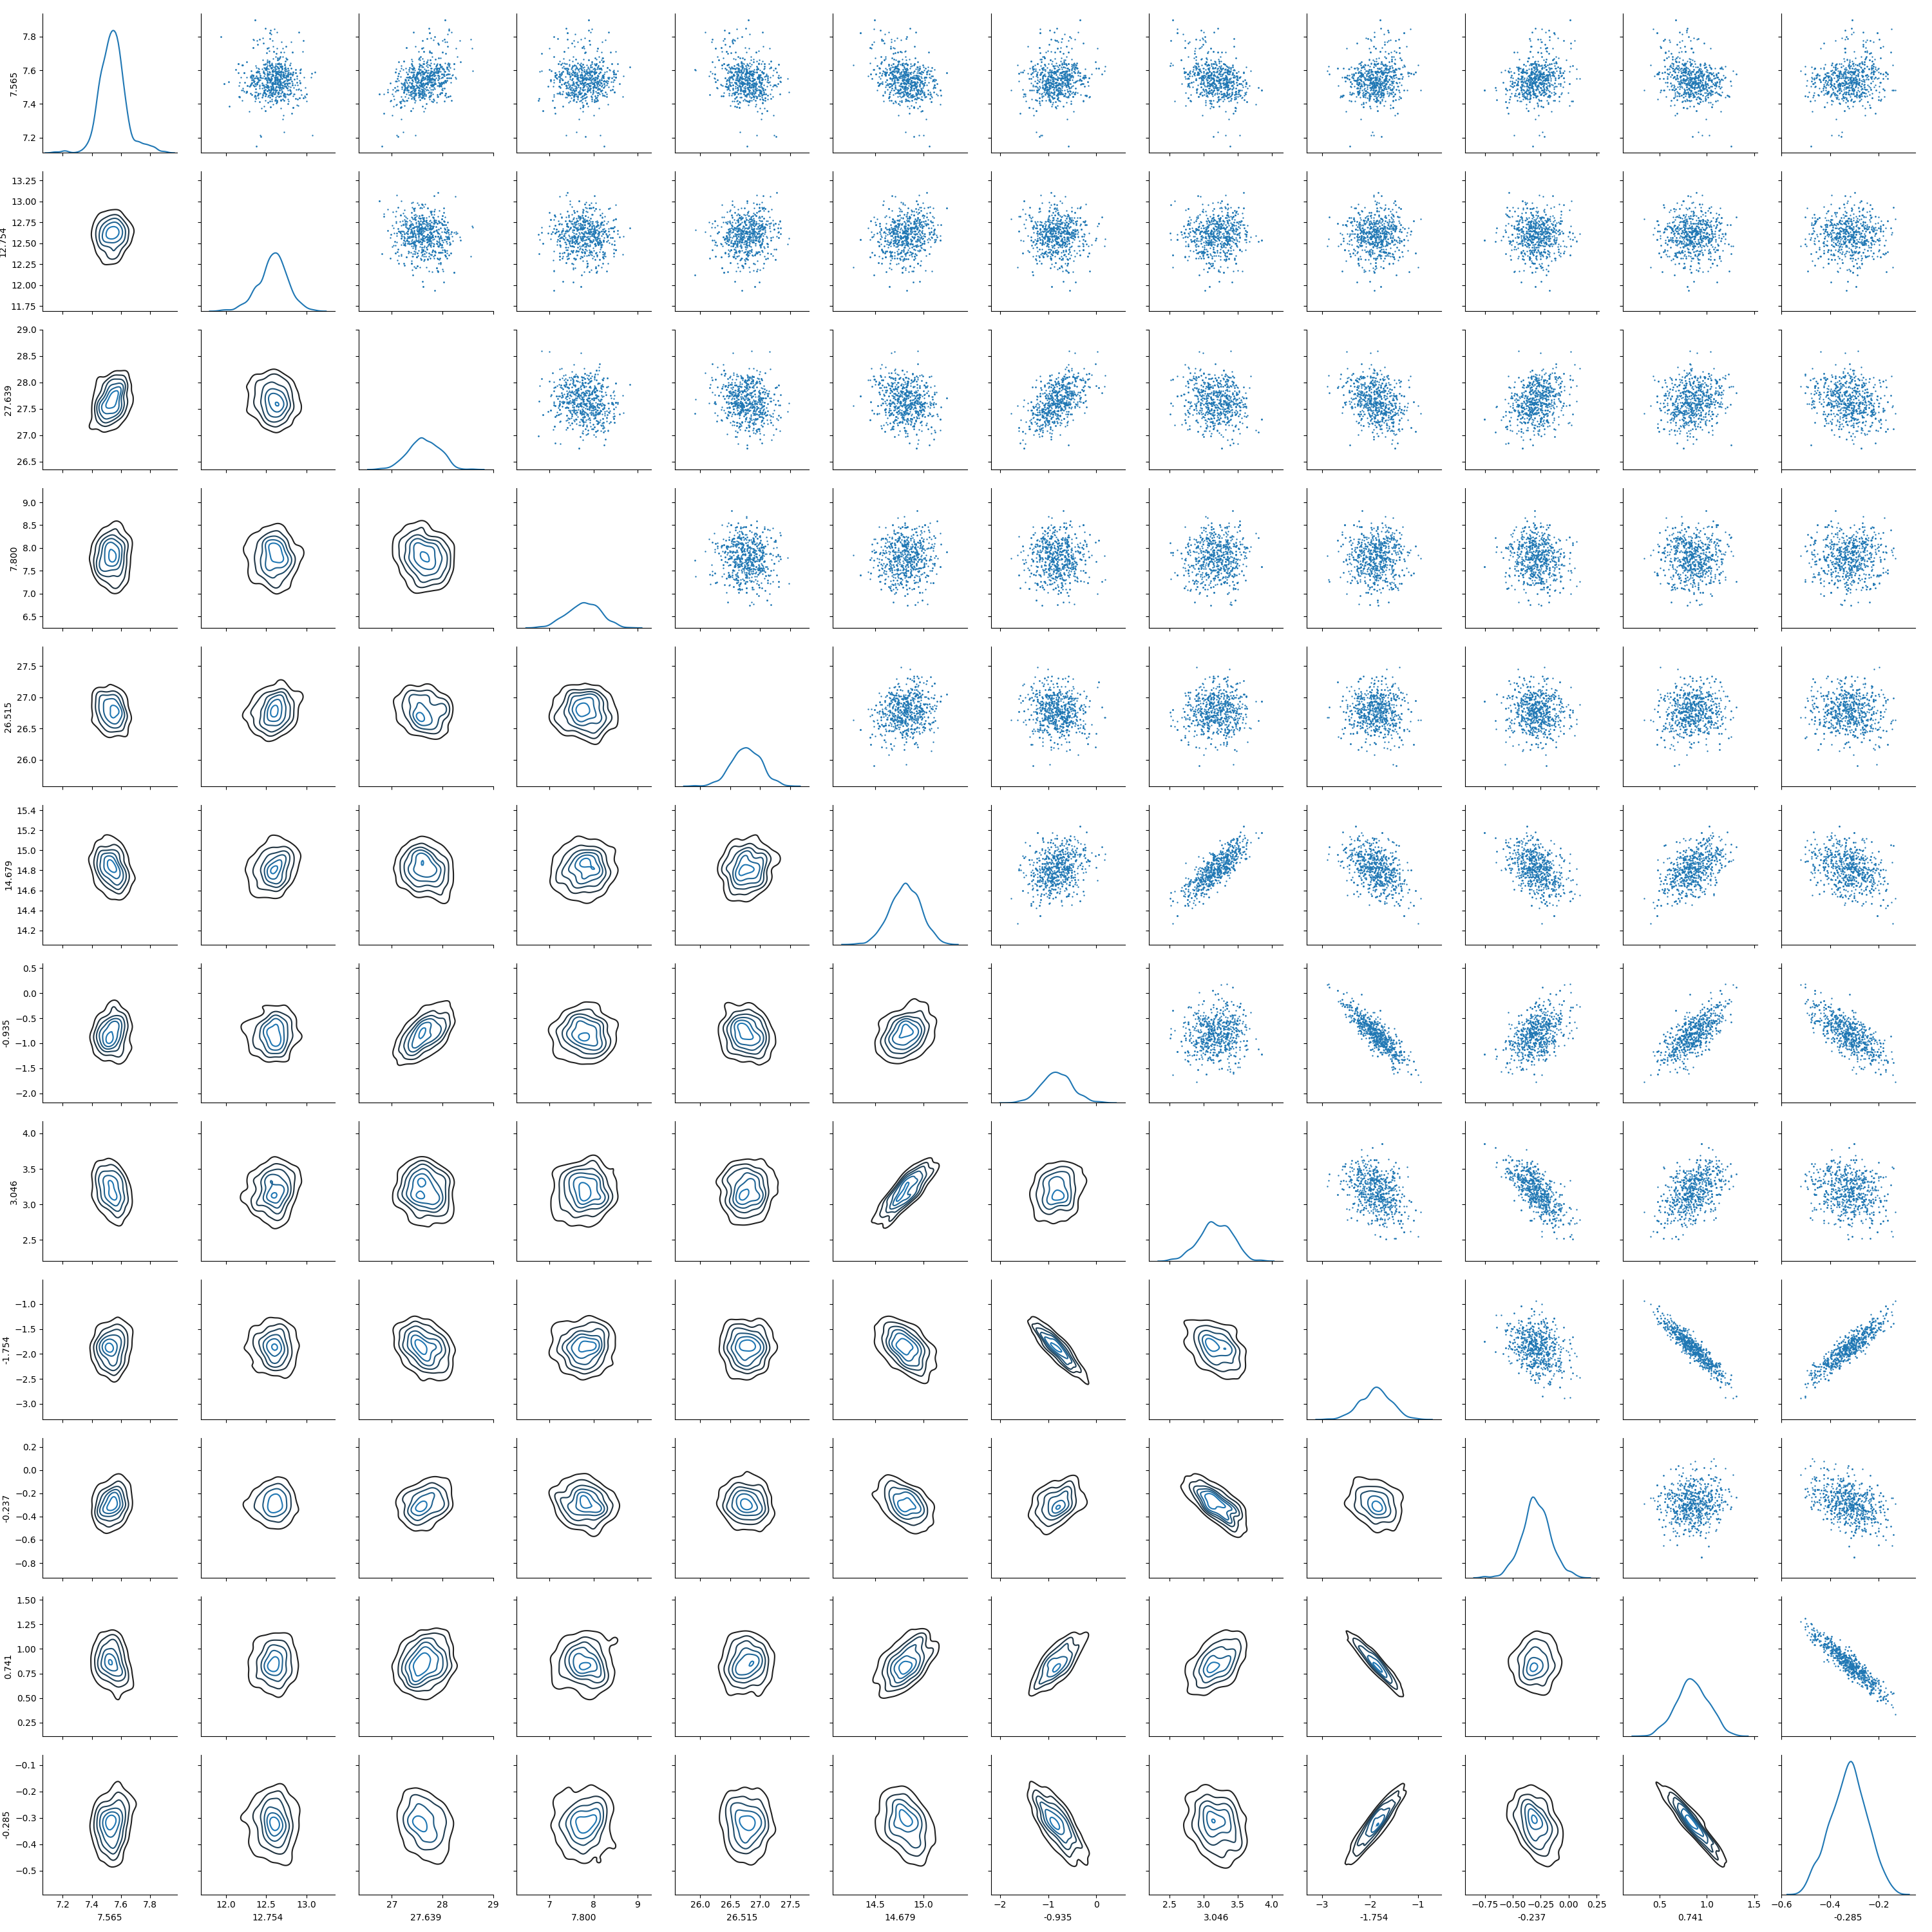
\includegraphics[width=1.0\textwidth]{../imgs/pairplot.png}
\end{minipage}
\caption{Маргинальные распределения параметров.}
\end{center}
\end{figure}



% У заключения нет номера главы
\pagebreak
\section*{Заключение}
\begin{enumerate}
        \item Выполнено обобщение на трехмерное поле скоростей метода \cite{NIIm} пространст\-вен\-но-кинематического моделирования однородной плоской подсистемы объектов Галактики, включающего оптимизацию сглаженности закона вращения и гибкий алгоритм исключения выбросов в данных. Метод применен к данным каталога звезд красного сгущения (ЗКС) APOGEE-RC DR-14 \cite{DRdata}.
        \item Сравнение оценок параметра Оорта $A$, полученных из анализа по отдельности поля лучевых скоростей и поля собственных движений по долготе, свидетельствует в пользу заниженности в среднем шкалы \cite{Laney} расстояний для ЗКС. Однако соответствующий поправочный коэффициент $K_A = 1.044 \pm 0.036$ незначимо отличается от единицы. Это следует учитывать при попытках применить такую перекалибровку к каталогу. Вместе с тем, благодаря большому объёму выборки ЗКС (свыше 29 тыс. опорных объектов), \textbf{впервые} удалось получить оценку $R_0$ с приемлемой точностью по долготным собственным движениям и гелиоцентрическим расстояниям до объектов. Превышение долготных оценок $R_0$ над оценками по лучевым скоростям поддерживает предположение о заниженности шкалы расстояний для ЗКС в каталоге APOGEE-RC DR-14. 
        \item Расстояние от Солнца до центра Галактики $R_0$, полученное в результате, составляет
                \begin{equation}
                        R_0 = 7.516^{+0.072}_{-0.090}|_{\mathrm{stat}} \pm 0.247 |_{\mathrm{calib}} ,
                \end{equation}
                c поправкой шкалы расстояний
                \begin{equation}
                        R_0 = 7.838^{+0.101}_{-0.088}|_{\mathrm{stat}} \pm 0.283 |_{\mathrm{calib}} .
                \end{equation}
                Получены оценки для всех фундаментальных параметров Галактики. Неопределенность результата дают систематические погрешности, статистические ошибки относительно малы. 
        \item Большая радиальная и вертикальная протяженность выборки позволила исследовать кинематику Галактики на значительном отрезке расстояний, и построить статистически точную среднюю кривую вращения на отрезке $\approx 12$ кпк в радиальном направлении. Построенная на интервале галактоцентрических расстояний $3-15$ кпк по трехмерному полю скоростей кривая вращения \textit{плоская} на отрезке от 6 до 14 кпк, с незначительным спадом (аналогично найденным в \cite{Rastorguev, Baikbob}). Значимость падения предполагается установить. Мелкомасштабной структуры кривой вращения \textit{не выявлено}.
\end{enumerate}
\setmonofont[Mapping=tex-text]{CMU Typewriter Text}
\pagebreak
\bibliography{diploma.bib}
\bibliographystyle{ugost2008ls}


%\pagebreak
%\section *{Приложение.}
%Кривые вращения для решения \ref{table_hsoy_sigma0} порядков $n=3, 4$.
%\begin{figure}[h!!]
%\begin{center}
%\begin{minipage}[h!!]{0.40\linewidth}
%        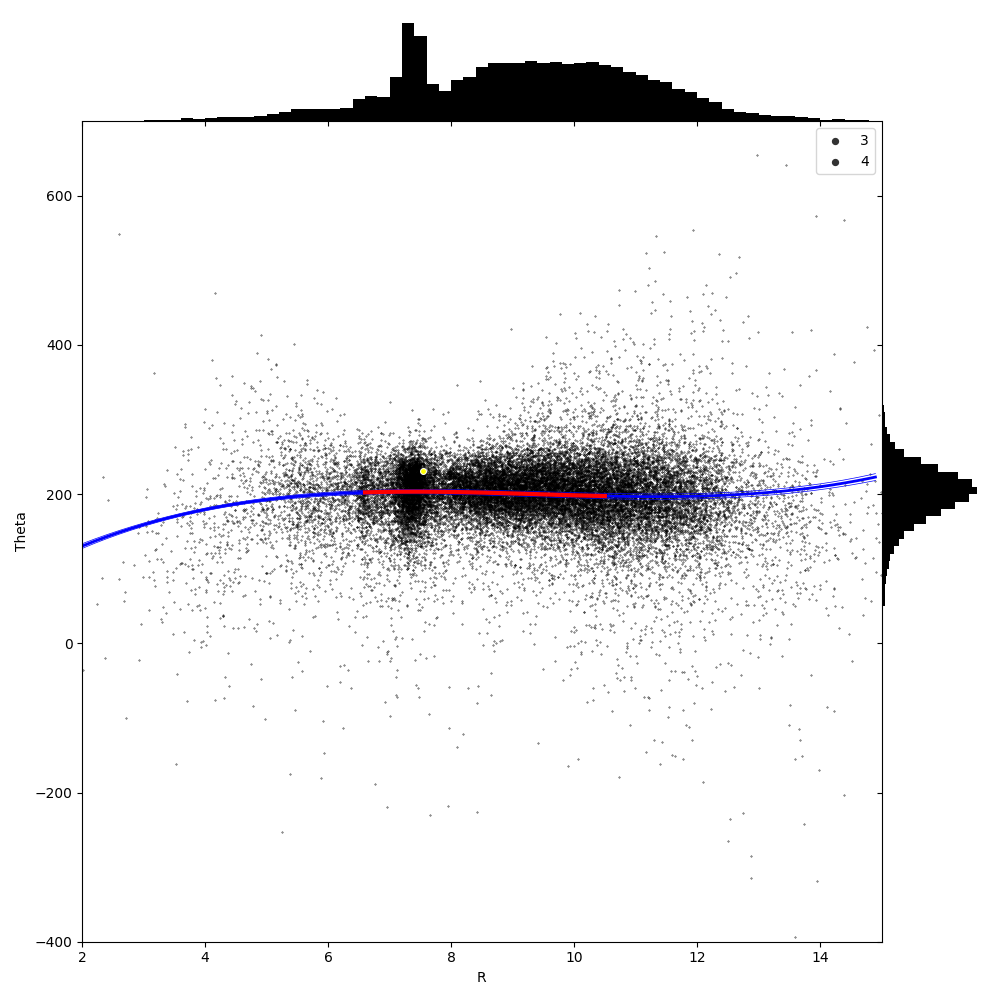
\includegraphics[width=1.0\textwidth]{../imgs/app/3.png}
%\end{minipage}
%\begin{minipage}[h!!]{0.40\linewidth}
%        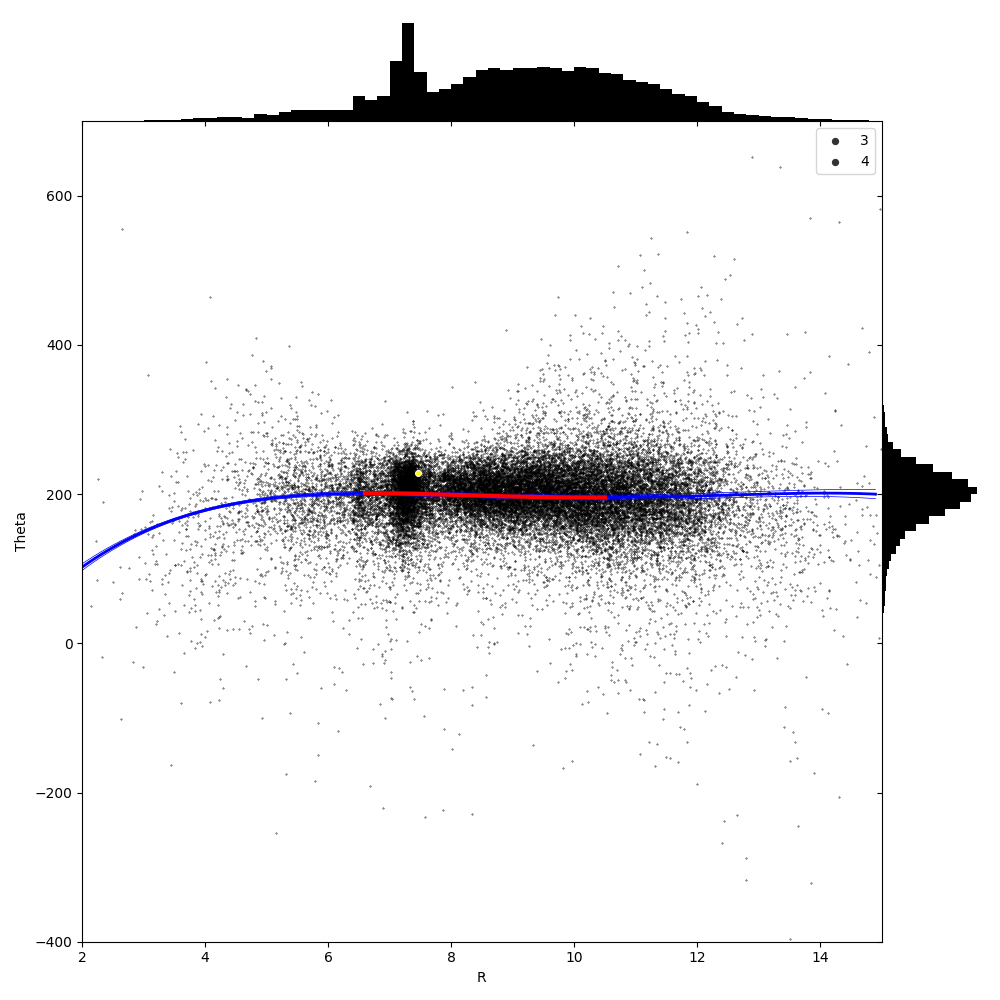
\includegraphics[width=1.0\textwidth]{../imgs/app/4.png}
%\end{minipage}
%\end{figure}
%\end{center}

\pagebreak
\section*{Приложение}
Пример нарушений связности линий равной плотности маргинальных распределений парамеметров для $n=4$ в \ref{table_hsoy_sigma0} (HSOY). Результаты Монте-Карло \ref{mk}, используемый ГПСЧ -- вихрь Мерсенна.
\begin{figure}[h!!]
\begin{center}
        \includegraphics[width=0.9\textwidth]{../defpair.png}
\end{center}
\end{figure}

\end{document}
